\section{Hardware}
\label{Hardware}

As explained in \cref{Concept}, the device can be divided into four parts. This section will explore each separately by looking into the circuits, housing and all the design choices that led to the finished product. \\


\subsection{The Ignition Voltage Generator}
\label{Ignition Voltage Generator}

\begin{figure}[!ht]
    \centering
    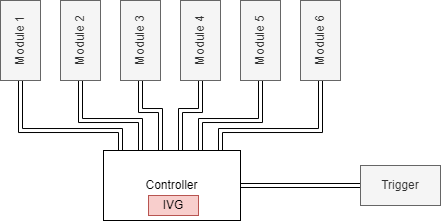
\includegraphics[width=5cm]{./Figures/concept_ivg.png} 
\end{figure}

\noindent The ignition voltage generator shown in \cref{fig:ivg_circuit} works by the basic principle of a step-up/boost converter, by storing energy in form of a magnetic field inside an inductor and releasing the energy as a current into a capacitor. Repeat this process at a high frequency and a high voltage is generated at the output. For a detailed explanation please read the document about this topic by \textit{Texas-Instruments}\footurl{https://www.ti.com/lit/an/snva731/snva731.pdf}.


\subsubsection{Circuit}

\begin{figure}[!ht]
    \centering
    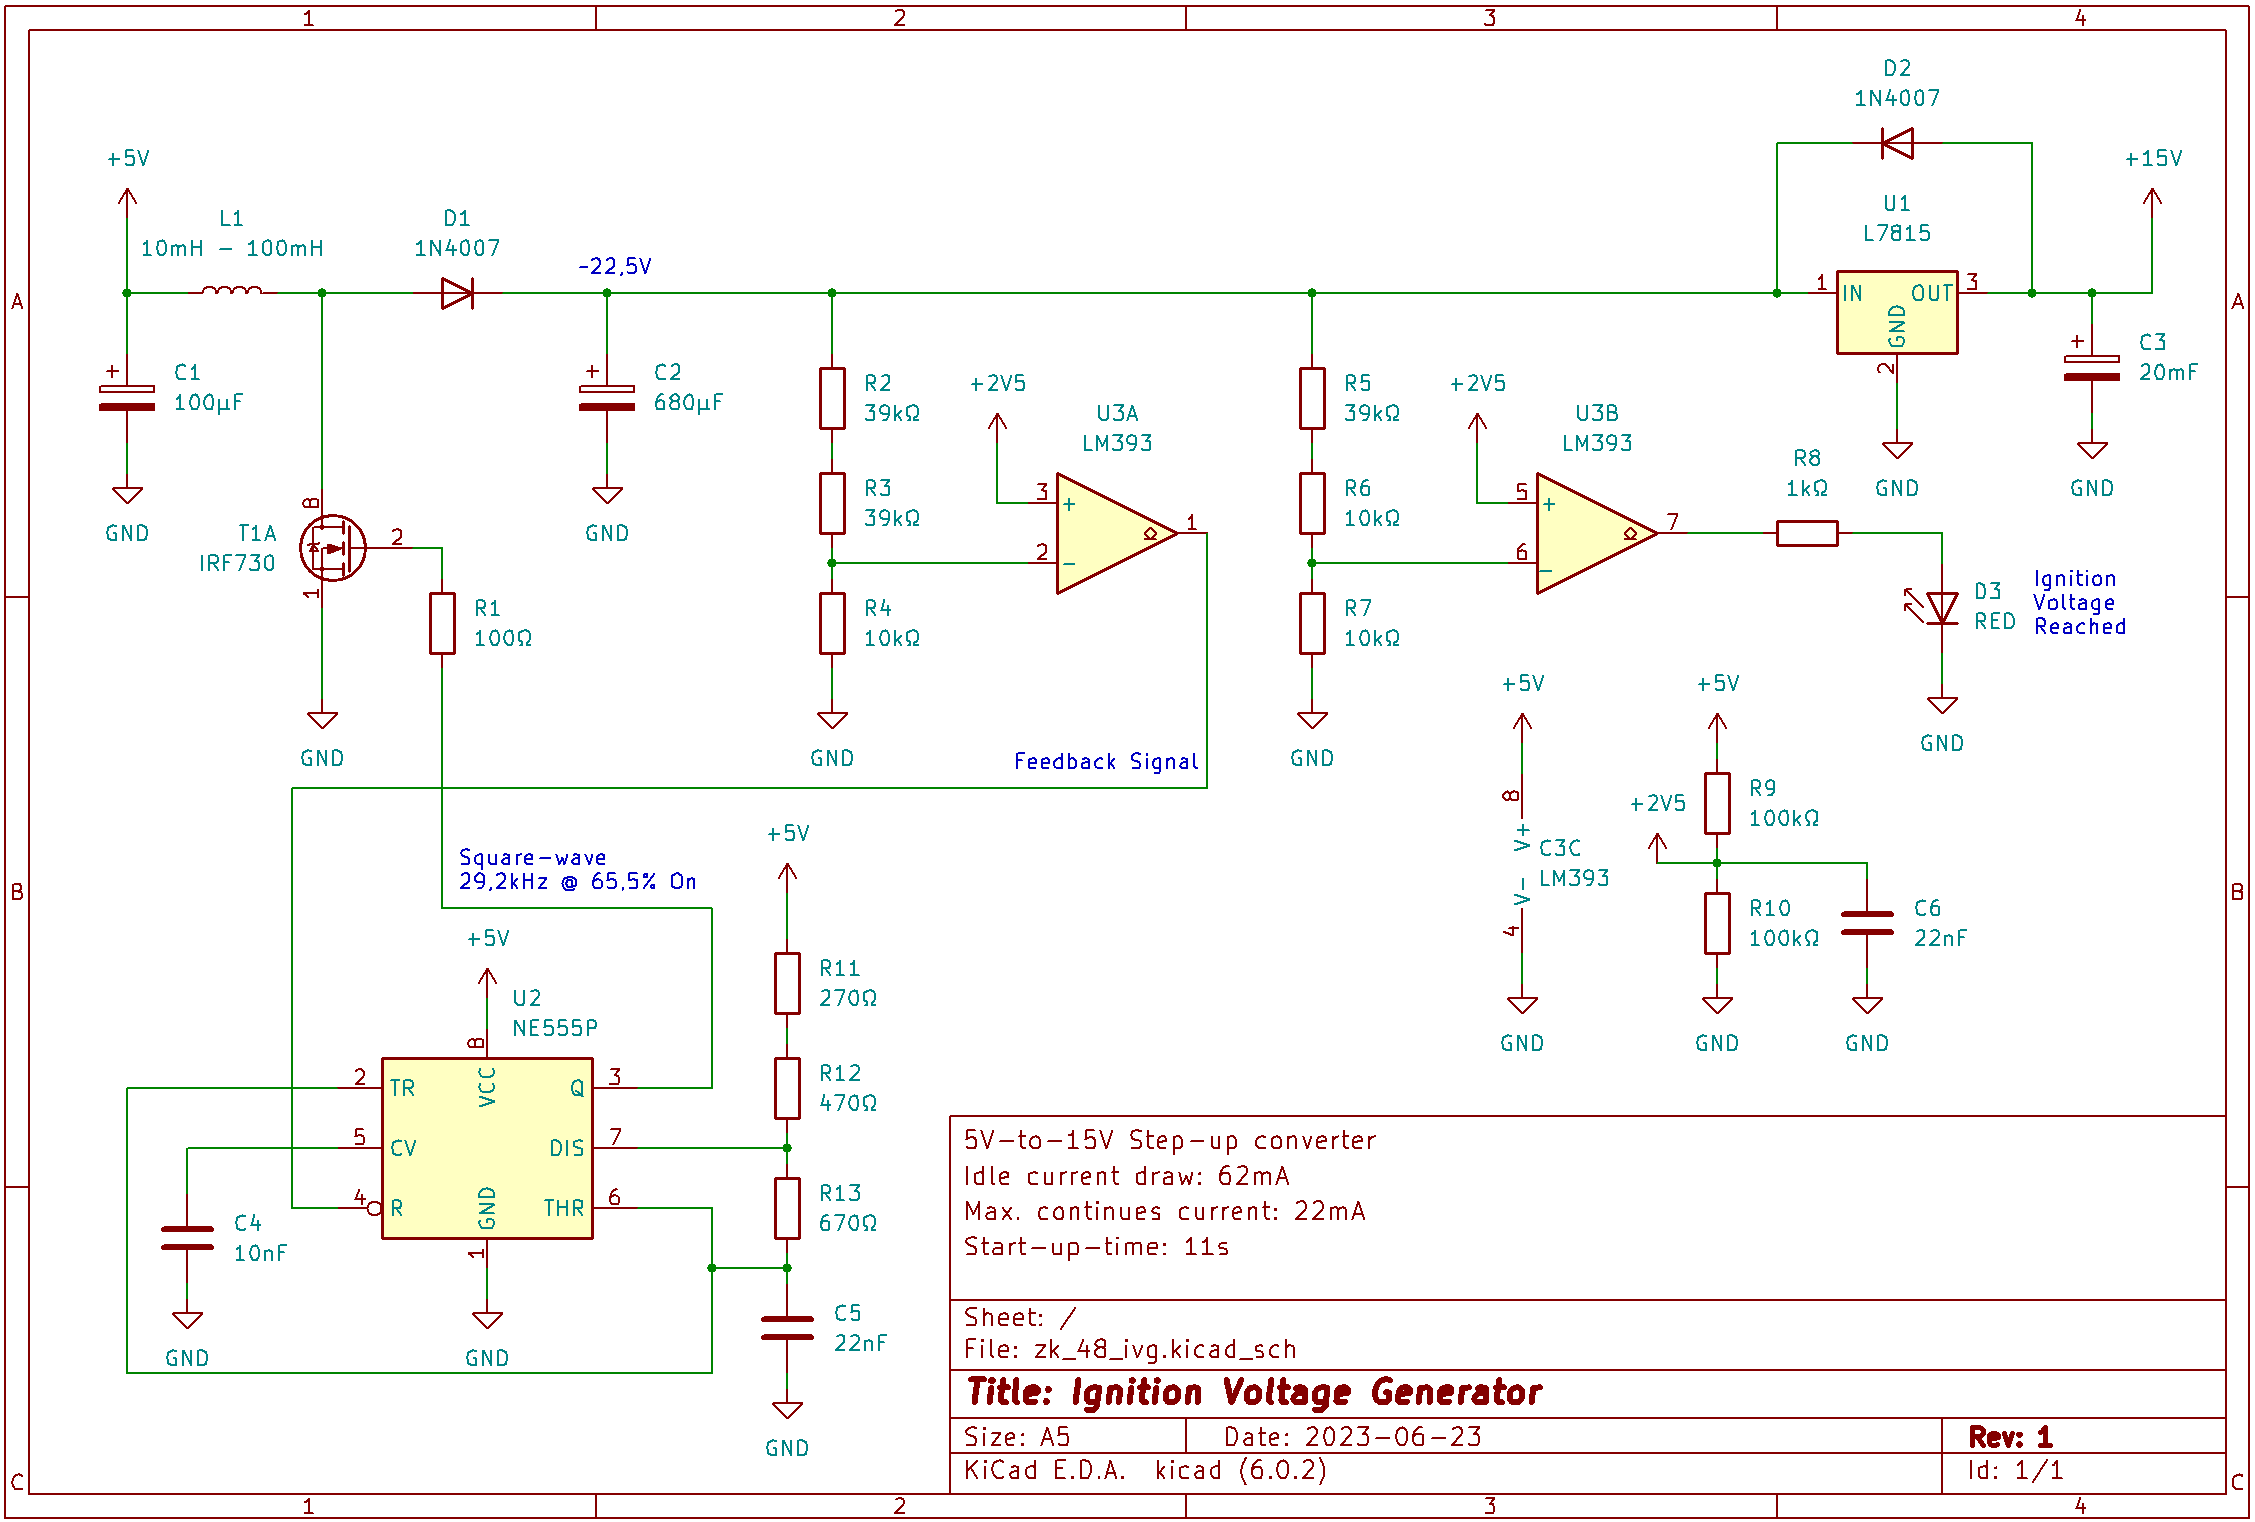
\includegraphics[width=15cm]{./Figures/ivg_circuit.png}
    \caption{Circuit of the 5V-to-15V step-up converter.}
    \label{fig:ivg_circuit}     
\end{figure}

\pagebreak

\subsubsection{How does the circuit work?}

\noindent The circuit shown in \cref{fig:ivg_circuit} is based on the popular NE555\footurl{ https://www.ti.com/lit/ds/symlink/ne555.pdf}, the dual voltage comparator LM393\footurl{https://www.ti.com/lit/ds/symlink/lm393.pdf} and the fixed $15V$ linear voltage regulator L7815\footurl{https://www.st.com/resource/en/datasheet/l78.pdf}. The NE555 is used as a square wave oscillator to generate a $29,2kHz$ $5V_{pp}$ signal with a $65,5\%$ on-time. This signal drives the IRF730\footurl{https://www.vishay.com/docs/91047/91047.pdf} N-channel MOSFET, which switches current through the inductor $L1$ and therefore charging the capacitor $C2$. This voltage is named the intermediate voltage.\\

\noindent Through a voltage divider the voltage at $C2$ is stepped down by a factor of $\frac{1}{9}$ and compared to a $2,5V$ reference voltage by $U3A$. This results in a $5V$ output signal at the output of $U3A$, if the capacitors $C2$ voltage is lower than $22,5V$. This signal is called the feedback signal and is used to turn off the NE555, if the intermediate voltage has reached $22,5V$. Using a schmitt-trigger results in a oscillating feedback signal, which is undesirable in this configuration. If the intermediate voltage reaches $22,5V$, the feedback signal will no longer be $5V$ or $0V$, instead it will drop to a constant $2,5V$. This is expected as no schmitt-trigger is used, but will result in unpredictable behaviour by the NE555, as it expects a binary reset signal. This seems like a problem, but in reality will result in the NE555 output voltage to drop below the on-voltage of the IRF730, thus turning it off. It is also observable that the frequency and on-time of the NE555 output is rising, but this has no effect, because the voltage already dropped significantly to turn off the MOSFET. \\

\noindent The intermediate voltage is then converted by the L7815 to stable $15V$, which charges the large $20mF$ ignition capacitor $C3$. This voltage is called the ignition voltage. \cref{eq:power_in_system} calculates the total energy stored in the system with all six modules connected (Thus the total capacitance being $26mF$, but read more in \cref{Ignition Module work} "Additional circuits") which equates to around $3J$ and therefore does not pose any  danger to life\footurl{https://www.ehss.vt.edu/programs/ELR_capacitors.php}. Touching the fully charged capacitors with wet hands (which is highly advised against doing!) did not result in any shock or pain.\\

\begin{equation}
W_{el}=\frac{U^2 \cdot C_{tot}}{2}=\frac{(15V)^2 \cdot 26mF}{2}=2,925J
\label{eq:power_in_system}
\end{equation}\\

\noindent The second comparator $U3B$ in the LM393 package is used to turn on a red signal LED $D3$, whose purpose is to indicate whether the intermediate voltage is bigger than $14,75V$. This shows the user if the system is ready for operation and if ignition voltage is present.\\


\pagebreak

\subsubsection{Testing}
\label{Testing}
For testing the ignition voltage generator, displayed in \cref{fig:ivg_circuit}, a resistor with $4,7\Omega$ was placed into port 1 on module 1 (Please read \cref{Ignition Module work} for further information about the circuit shown in \cref{fig:testrig_pulse}). This resistance is about equal of two bridge wire detonators connected in series. A lower resistance would strain the ignition voltage more, but often more than one detonator is used in a pyrotechnic show, thus making it a bit more realistic. \Cref{fig:testrig_pulse} shows the complete test setup, with the pulse generator symbolically representing the controller. The system was programmed to fire(one fire pulse takes $10ms$) port 1 on module 1 eight times with a $10ms$ delay between each pulse.

\begin{figure}[!ht]
    \centering
    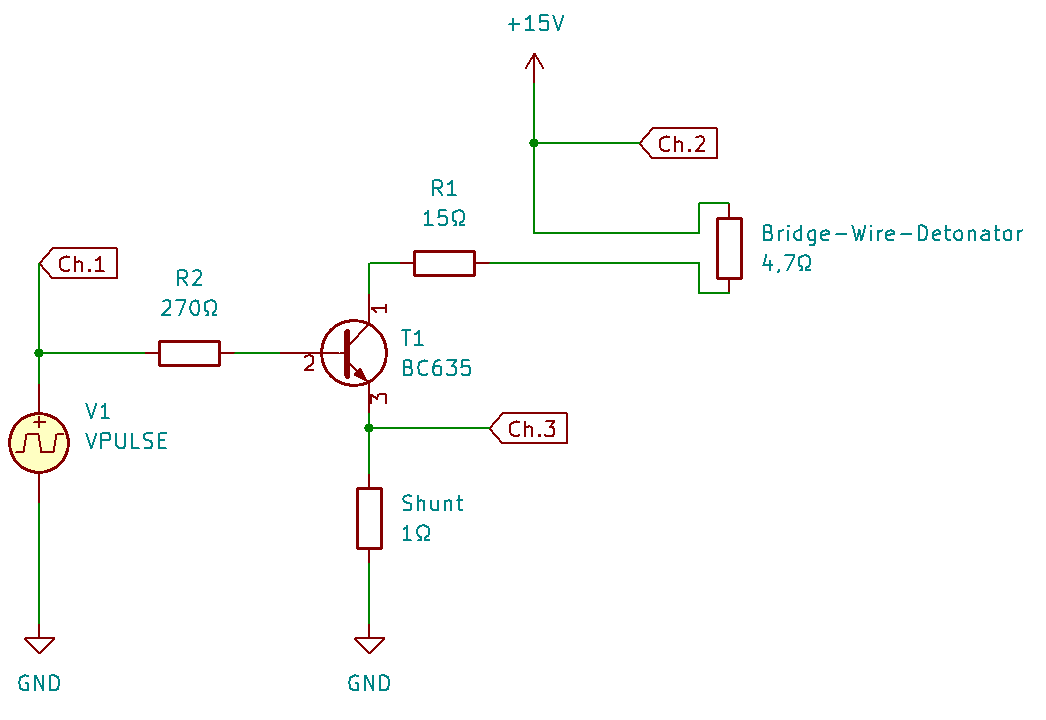
\includegraphics[width=7cm]{./Figures/testrig_pulse.png}
    \caption{Circuit for testing stability of ignition voltage and current through a simulated bridge wire detonator.}
    \label{fig:testrig_pulse}     
\end{figure}

\paragraph{Results}
\label{Results}

\noindent The first test consisted of 8 pulses to simulate fast consecutive firing of pyrotechnic single-shots\footurl{https://www.youtube.com/watch?v=UgVG9NcA5CM} or other pyrotechnic effects. Normally firing the same port multiple times does not make sense, but for testing purposes this is equivalent to firing eight separate ports. The resulting waveform was captured with the Quad DSO (digital storage oscilloscope) \textit{Rigol DS1054z}\footurl{https://www.batronix.com/pdf/Rigol/UserGuide/DS1000Z_UserGuide_EN.pdf}.\\

\begin{figure}[!ht]
    \centering
    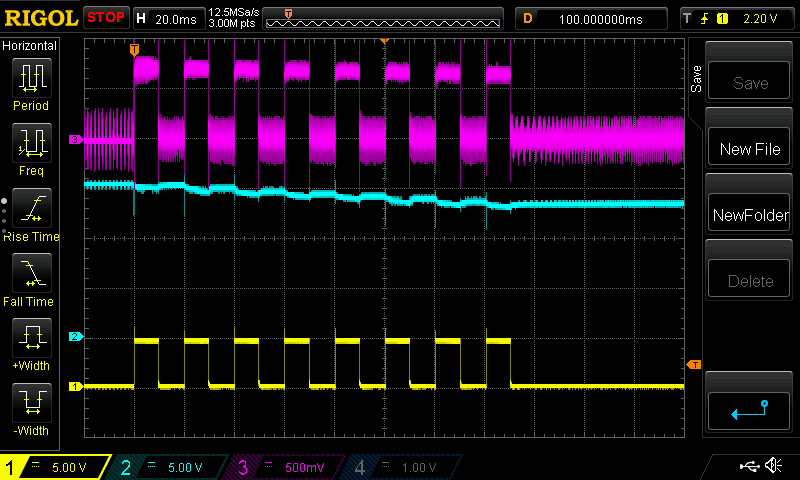
\includegraphics[width=10cm]{./Figures/eight_pulses_close.png}
    \caption{The recorded waveforms by the oscilloscope of eight pulses in close up.}
    \label{fig:eight_pulses_close}     
\end{figure}
 
\noindent The main objective of this test was confirming that rapid firing does not affect the systems ability to ignite further detonators. This can evidently be confirmed by looking at the curve of Ch.3 and Ch.2 in \cref{fig:eight_pulses_close}. The ignition voltage is represented by Ch.2 which drops only by $2V$, thus being neglectable. By looking at Ch.3, which shows the current through the bridge wire detonator, it is noticeable that the current is above $700mA$, even at the last pulse. Past testing showed, bridge wire detonators already ignite at around $300mA-400mA$. This confirms the efficacy and the systems ability to continuously ignite pyrotechnic effects at a high rate.

\pagebreak

\noindent In \cref{fig:eight_pulses_wide} the time was measured for the ignition voltage to return back to $15V$ after firing eight times. This time amounts to about $2s$ which is acceptable, but could be improved.\\ 

\begin{figure}[!ht]
    \centering
    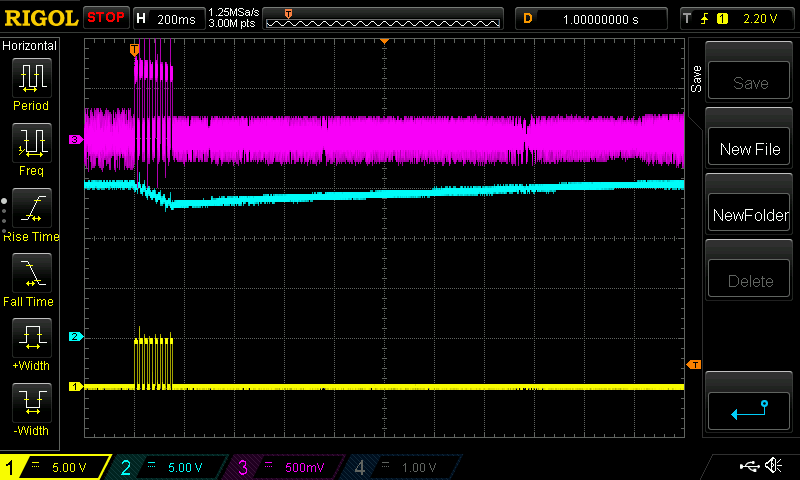
\includegraphics[width=10cm]{./Figures/eight_pulses_wide.png}
    \caption{The recorded waveforms by the oscilloscope of eight pulses, until the ignition voltage returns to $15V$.}
    \label{fig:eight_pulses_wide}     
\end{figure}

\noindent The third test focused on finding the absolute limit of the system. To achieve this objective the ZK-48 was programmed to use all its 48 sequence slots and fire port 1 on module 1 48 times. 

\begin{figure}[!ht]
    \centering
    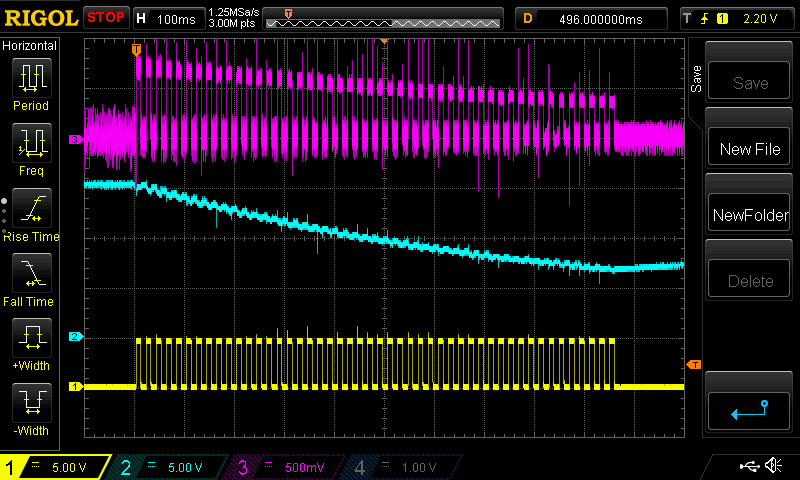
\includegraphics[width=10cm]{./Figures/max_pulses.png}
    \caption{The recorded waveforms by the oscilloscope of 48 firing pulses.}
    \label{fig:max_pulses}     
\end{figure}

\noindent The maximal number of firing pules was determined by counting the number of pulses until the current through the detonator fell below $500mA$. This current value was chosen because it is the average between the lowest recorded current at which a detonator ignites($300mA$) and the current at the first ignition pulse($700mA$). By this definition, the maximal number of consecutive firing pulses with $10ms$ delay is about 24.

\paragraph{Conclusion}
The ignition voltage generator is able to provide a steady voltage, even under load(See \cref{fig:testrig_pulse}) and is able to ignite 24 bridge wire detonators consecutively with a $10ms$ delay. This is just theoretical and needs to be confirmed with real detonators, however this is already a good indicator for proper operation. Although the ignition voltage generator performs acceptably, it has many flaws and should be subject of rigorous optimization. For example, the ignition voltage should ideally not drop at all and remain constant even if continues $700mA$ are drawn. By using a bought step-up converter, with proper control logic, such as current regulation, instead of a simple feedback loop, most problems would be rectified. This projects goal is not buying electronic modules and soldering them together, instead this is an exploration of circuit design and should be viewed as a learning experience.


\pagebreak


\subsection{Controller}
\label{Controller}

\begin{figure}[!ht]
    \centering
    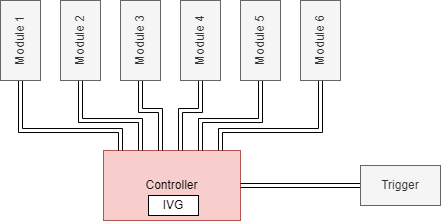
\includegraphics[width=5cm]{./Figures/concept_controller.png} 
\end{figure}

\noindent The controller is responsible for interpreting all user inputs such as the arm switch, the trigger signal and more which are processed by the µC to correctly control all modules to fire the pyrotechnic show. The ignition voltage generator is also soldered onto the same physical circuit board as the controller, but more about that in \cref{Circuitboard}.

\subsubsection{Circuit}
\label{Ctrlcircuit}

\begin{figure}[!ht]
    \centering
    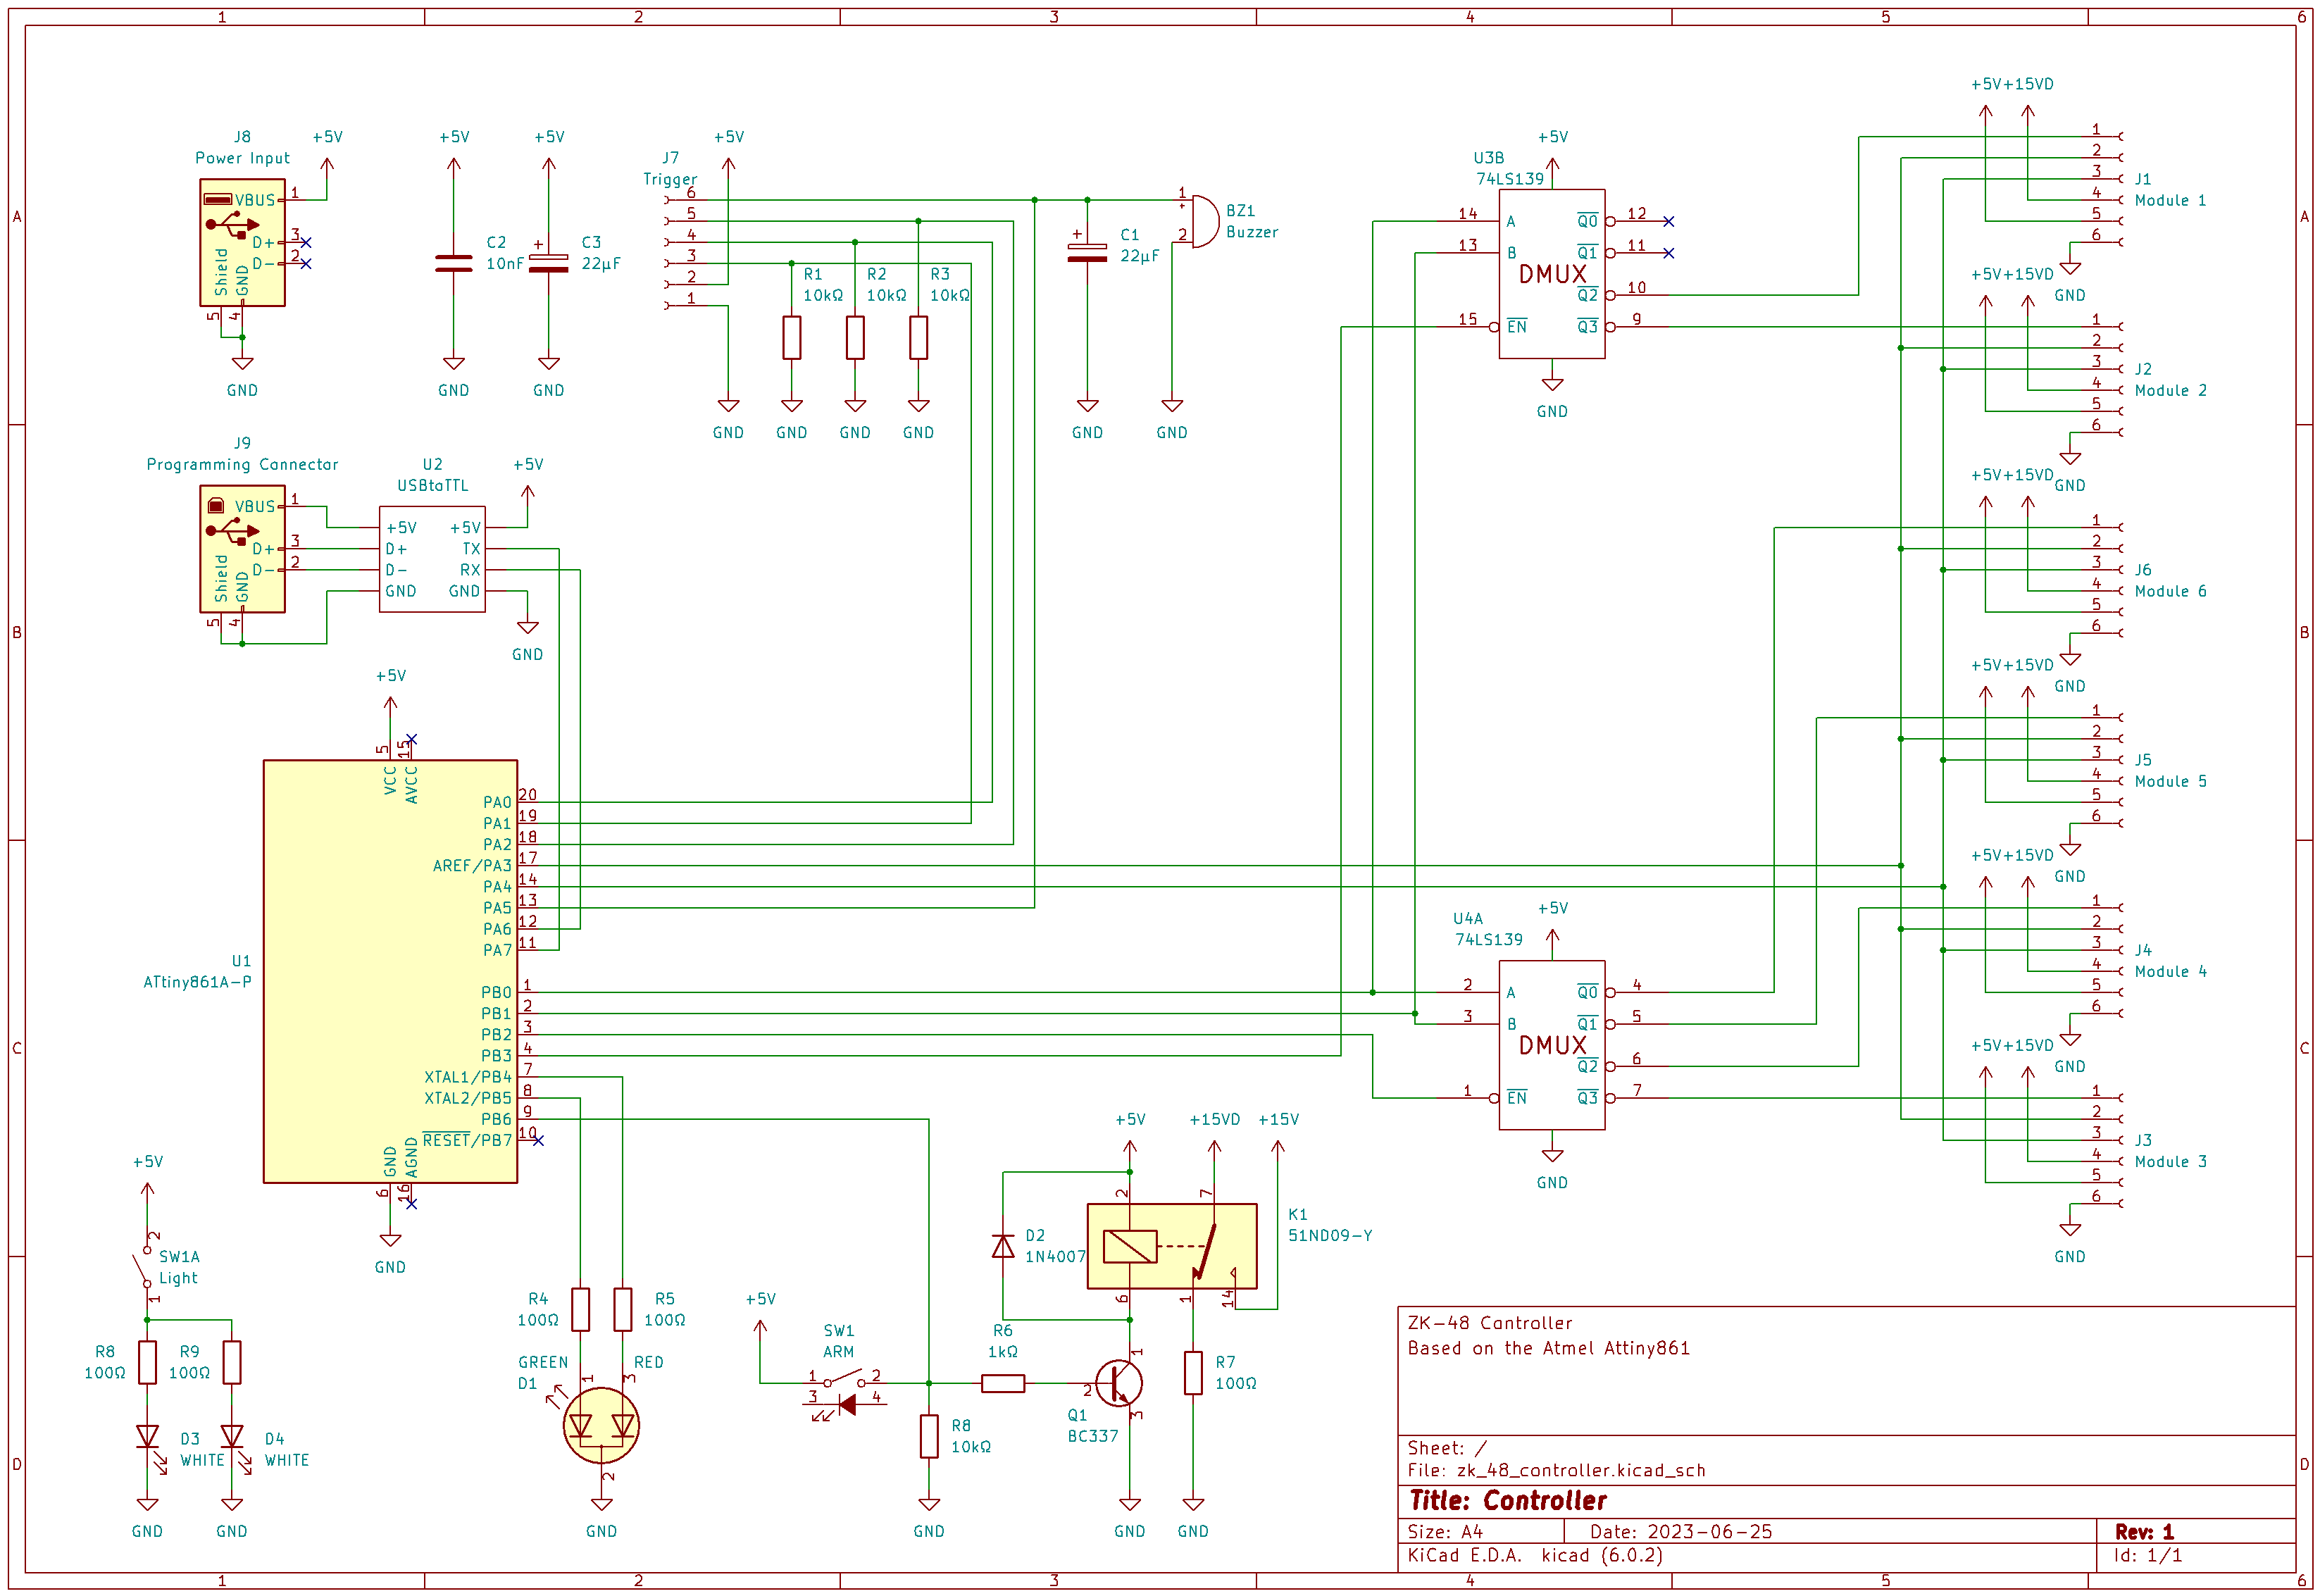
\includegraphics[width=15cm]{./Figures/controller_circuit.png}
    \caption{The circuit of the controller without ignition voltage generator.}
    \label{fig:controller_circuit}     
\end{figure}

\pagebreak

\subsubsection{Components of the Controller}
\label{Components of the Controller}
The controller consist of the peripheral managing and controlling logic, the USB serial communication and the arm safety circuit. 

\paragraph{Peripheral Managing and Controlling Logic}
This part of the circuit is located on the right side of the circuit depicted in \cref{fig:controller_circuit}. Its purpose is the selection of the correct ignition module to fire. To understand how this works, it is necessary to first explain how the µC fires a port on a module: In \cref{fig:controller_circuit} notice that all ignition modules sockets have their DATA and CLK lines connected together(For the pin-out see \cref{Sockets and Plugs}). First, the µC serially transmits to all modules shift registers, at the same time, the port that is about to be fired. In the second step, the µC selects one out of the six modules, which then fires the port that was set in the first step.\\

\noindent The selection process of the ignition module is accomplished by two demultiplexer $U4A$ and $U3B$ which are both contained in the dual DMUX 74LS139\footurl{https://www.ti.com/lit/ds/symlink/sn54ls139a-sp.pdf}. Instructions are given to the DMUX by the µC. This circuit design only allows to select one module at a time, thus the system is unable to fire two ports on different modules at the same time. Although the firmware does not support simultaneous firing of to ports anyway. This is a disadvantage, but is manageable by programming the system to fire two ports with no delay, which results in a $10ms$ between each firing. The human eyes cannot pick up on such short delays and pyrotechnics are also not timed perfectly, therefore this does not pose a problem.\\

\noindent The socket of the external trigger also falls into peripheral circuitry, but  it does not contain any logic. Resistors $R1-R3$ pull down the sockets FIRE, ARMED and CONCD lines(For the pin-out see \cref{Sockets and Plugs}). Those are inputs of the µC and are able to not have a defined potential, if the user unplugs the trigger when the system is powered on, therefore needing to be pulled down. The local signal buzzer $BZ1$ is wired to the sockets BUZZER signal and its voltage is stabilized by the capacitor $C1$. Without this capacitor, the sound of the buzzer is very unpleasant to the ear.\\

\paragraph{Attiny 861}
The heart of the controller is the 8-Bit AVR micro controller (µC) Attiny 861\footurl{https://www.mouser.com/datasheet/2/268/Atmel_2588_8_bit_AVR_Microcontrollers_tinyAVR_ATti-1315472.pdf}. Its most notable features are the 512 bytes in-system programmable EEPROM that stores the firing sequence, 16 I/O pins, the 8 kilobyte of program flash memory, as well as many more features. Further information will be provided in \cref{Firmware}.


\paragraph{USB serial communication}
For programming the firing sequence, the µC has to communicate with a computer. As the Attiny 861 does not have in-build UART support, the TTL serial communication was used instead. This requires a device that translates TTL to UART and back, which is often done by a FDTI chip\footurl{https://ftdichip.com/}. At the time where the hardware for this device was being build no FDTI chip or substitute chip could be obtained with reasonable pricing in the authors location. Therefore the decision was made to save time and money by buying a UART-to-TTL module of \textit{Amazon}. As this is a bought, which is against the spirit of this project, this module it will be replaced in the near future, when a FTDI chip is obtainable. \\

\begin{figure}[!ht]
    \centering
    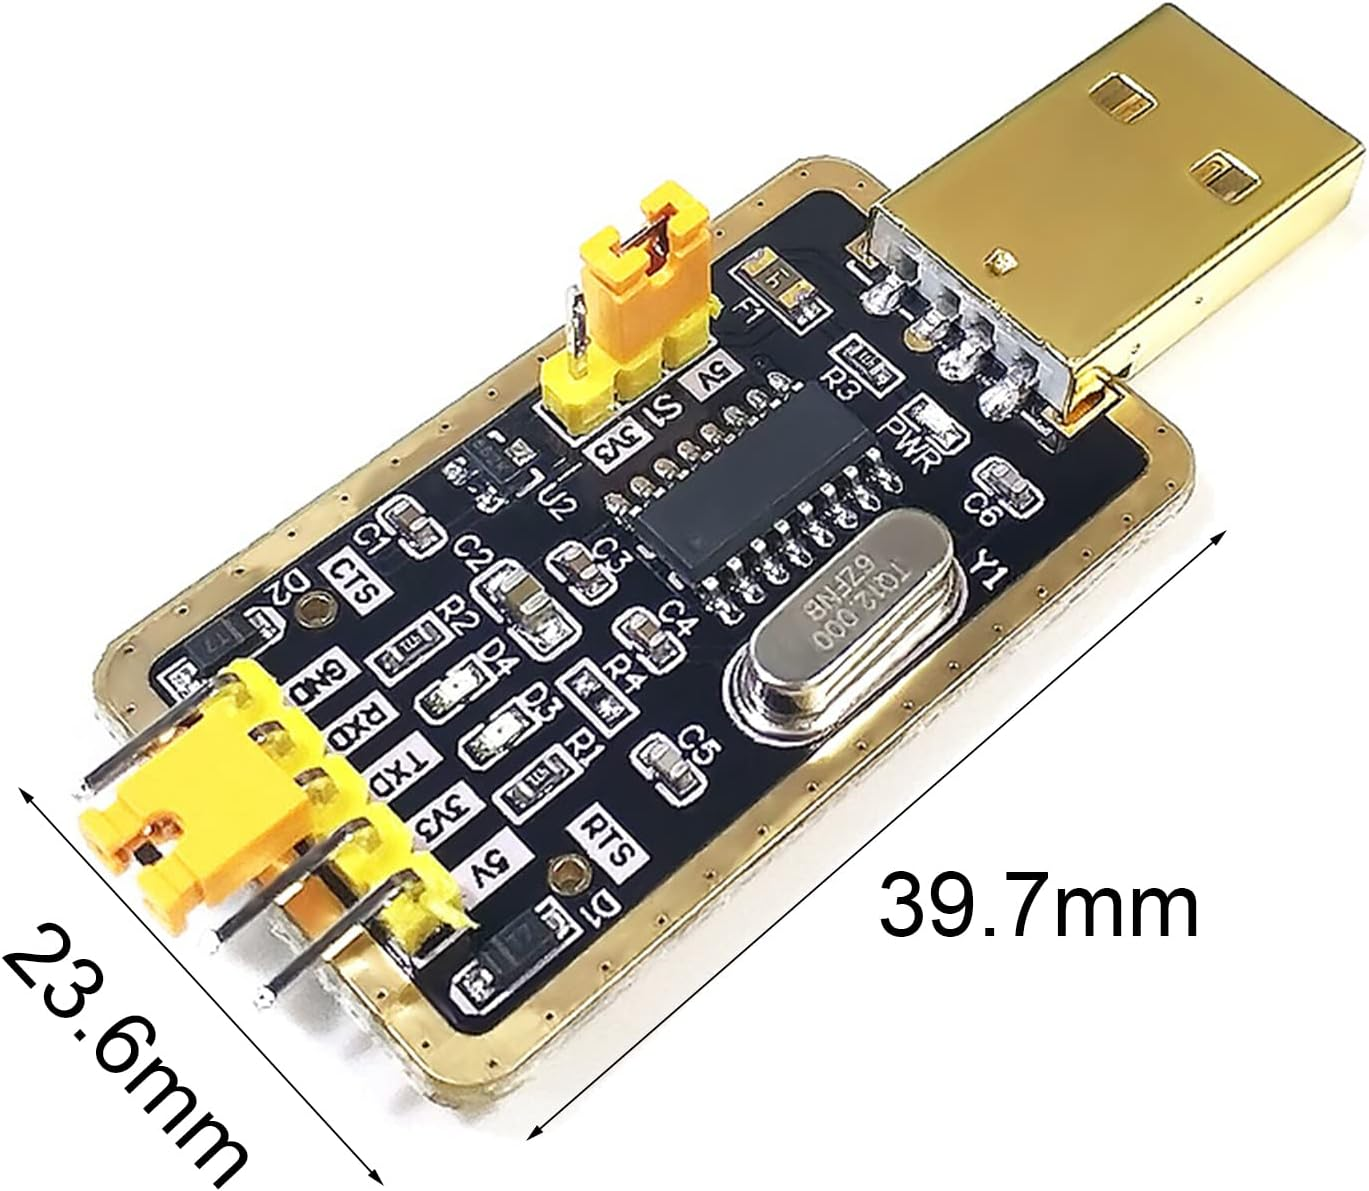
\includegraphics[width=3.5cm]{./Figures/uart_ttl.jpg}
    \caption{The bought UART-to-TTL converter from \textit{Amazon}}
    \label{fig:uart_ttl}     
\end{figure}

\sourceurl{}{fig:uart_ttl}{https://amzn.eu/d/3QKPgB9}

\pagebreak

\paragraph{Arm safety circuit}
This part of the controller circuit is shown in \cref{fig:controller_circuit} on the bottom and is very important. For safety reasons, the ignition voltage gets galvanically disconnected from the ignition voltage line of the modules, if the system is unarmed. Without this circuit, it is possible for a bridge wire detonator to ignite prematurely during power up or if a module is disconnected and reconnected. \\

\noindent The cause of this very dangerous behaviour is explained by the shift registers used in the ignition modules(See \cref{Ignition Modules}). Most shift registers will, when connected to power, take on random values inside their internal registers. If the output is disabled through the \textit{Output Enable} pin on the 74HC595(For further information see \cref{Ignition Module work} "Controlling the Ignition Circuits"), this could not happen. However those enable pins are driven by the DMUX on the controller (See \cref{fig:controller_circuit}) and those DMUX are controlled by the µC. But a µC takes a lot longer to boot than a shift register. Thus for a very short period ($<20µs$) of time, turning on random outputs of the shift registers and making premature ignition possible.\\

\noindent Although this cannot be prevented in the firmware, it is possible to remove the ignition voltage and pulling down the modules ignition voltage line with a $100\Omega$ resistor (See resistor $R7$ in \cref{fig:controller_circuit}). The relay $K1$ is only connecting the ignition voltage to the modules power lines, if the controller arm switch is physically toggled on and therefore making it near impossible to accidentally set of pyrotechnics unintentionally.

\paragraph{Additional circuits}
As the system will most likely be operated in the dark, the decision was made to add a small LED light inside the casing of the controller, to illuminate the interface. The circuit can be found in the bottom left corner in \cref{fig:controller_circuit}, although the LEDs are not soldered onto the circuit-board. They are placed inside the lid(See \cref{Housing of the Controller}), shining downwards on the interface.

\subsubsection{Sockets and Plugs}
\label{Sockets and Plugs}

\begin{figure}[!ht]
    \centering
    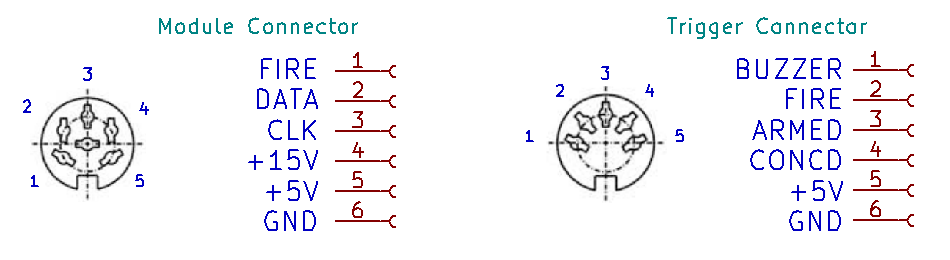
\includegraphics[width=10cm]{./Figures/mod_trig_connector.png}
    \caption{The pin-out of the trigger and modules socket/plug.   }
    \label{fig:mod_trig_connector}     
\end{figure}

\sourceurl{the socket sympol in}{fig:mod_trig_connector}{https://cdn-reichelt.de/documents/datenblatt/C160/MAB\%205S-ROHS_XX.pdf}


\noindent To connect the peripheral devices to the controller DIN\footurl{https://en.wikipedia.org/wiki/DIN_connector} plugs and sockets were used. The module socket and plug where chosen differently than the triggers, because accidentally plugging the trigger into a module socket would damage the triggers electronics. For the pin-out of each socket see \cref{fig:mod_trig_connector} and below in \cref{fig:din_plug_socket} the modules socket and plug is visible.

\begin{figure}[!ht]
    \centering
    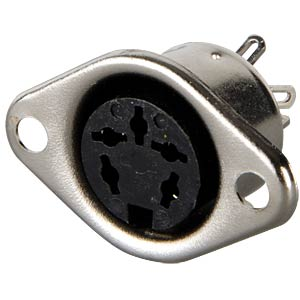
\includegraphics[width=3cm]{./Figures/MAB_5.jpg}
    \hspace{2cm}
    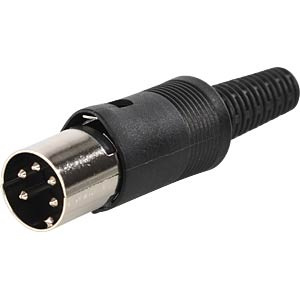
\includegraphics[width=3cm]{./Figures/MAS_50.jpg}
    \caption{The DIN socket and plug of the modules.}
    \label{fig:din_plug_socket}     
\end{figure}

\sourceurl{}{fig:din_plug_socket}{https://cdn-reichelt.de/bilder/web/xxl_ws/C160/MAS_50.png}
\sourceurl{}{fig:din_plug_socket}{https://cdn-reichelt.de/bilder/web/xxl_ws/C160/MAB_5.png}

\pagebreak

\subsubsection{Circuit board}
\label{Circuitboard}

\noindent A perfboard with one sided solder copper pads with the dimensions of 100x115mm was used as the base for the controller circuit. Both the controller circuit (See \cref{fig:controller_circuit}) and the ignition voltage generator (See \cref{fig:ivg_circuit}) were soldered onto the same board. Ideally, a PCB should be used to improve EMC, but this would make it difficult to change things in the future. \\

\begin{figure}[!ht]
    \centering
    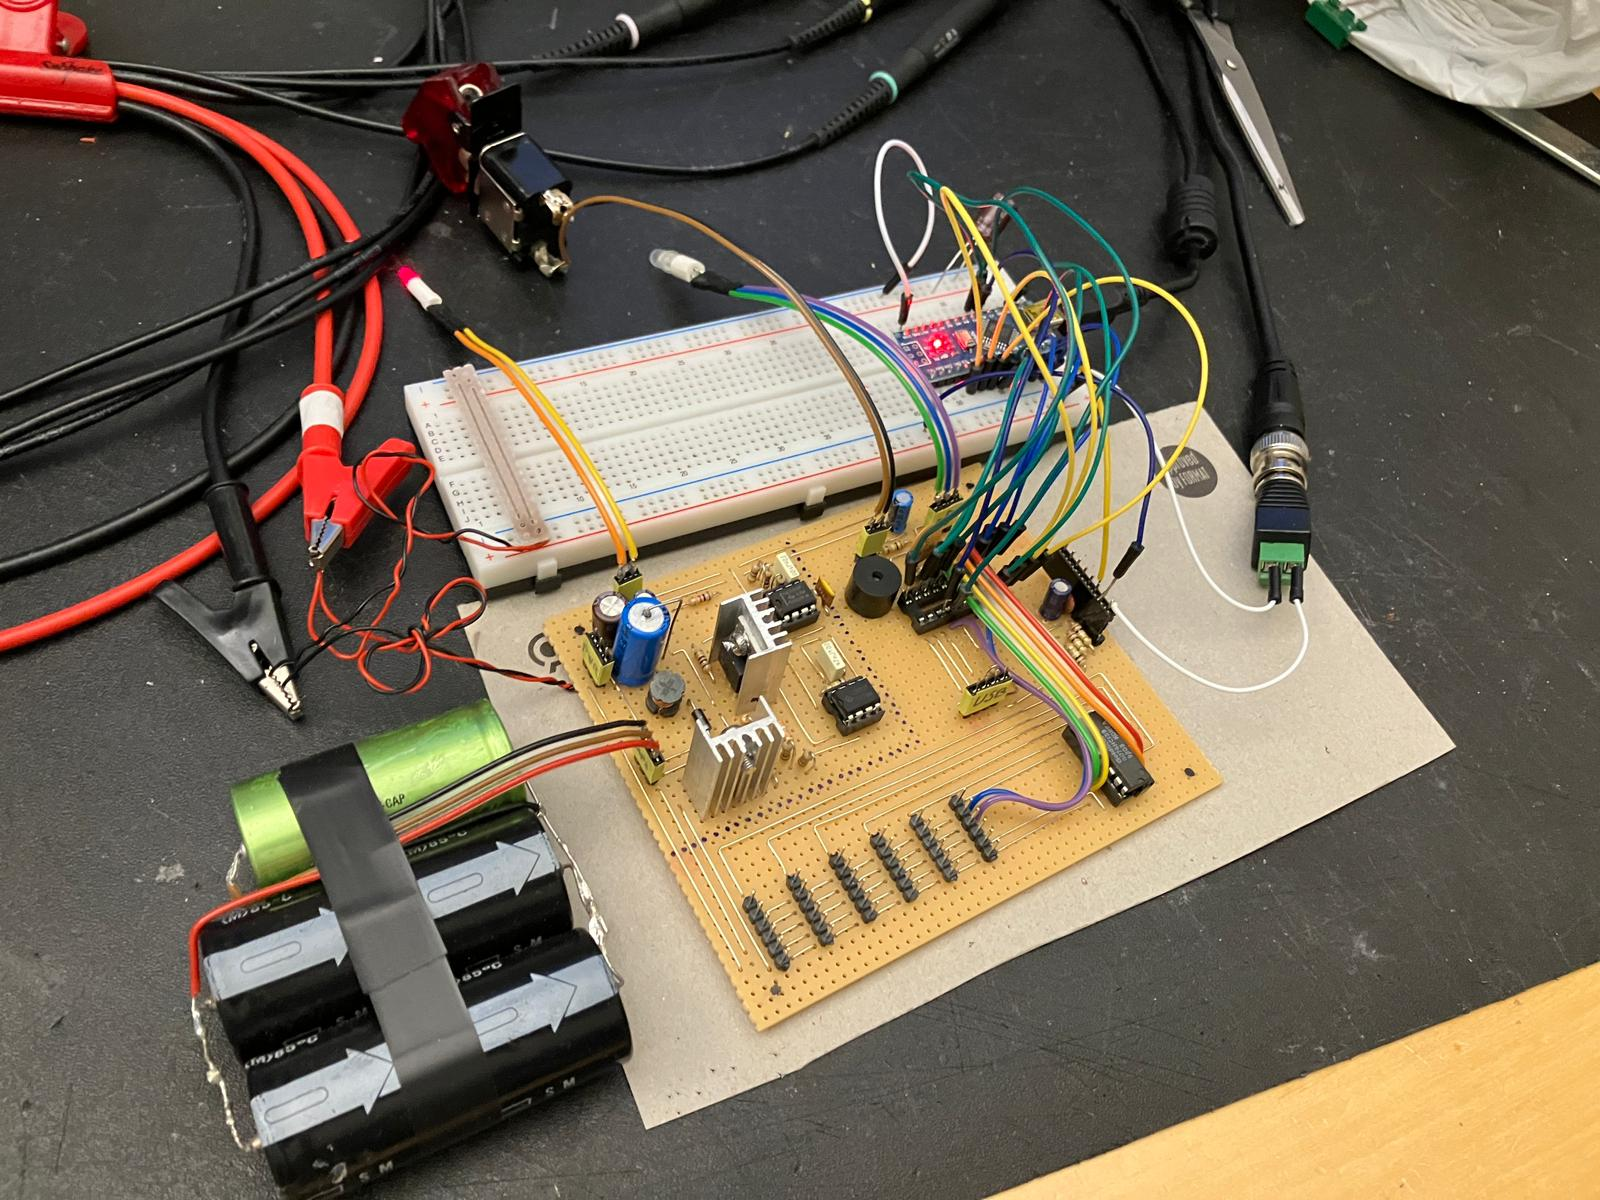
\includegraphics[width=10cm]{./Figures/dev_controller.jpeg}
    \caption{The controller circuit during development.}
    \label{fig:dev_controller}     
\end{figure}

\noindent The ignition voltage generator is visible in the left top corner, with heat sinks mounted onto the MOSFET and voltage regulator. The right top corner contains the µC, all the pin-headers for connecting the switches, LEDs and the arm safety circuit. On the bottom, the peripheral managing logic is visible together with the six pin-headers for the modules.

\begin{figure}[!ht]
    \centering
    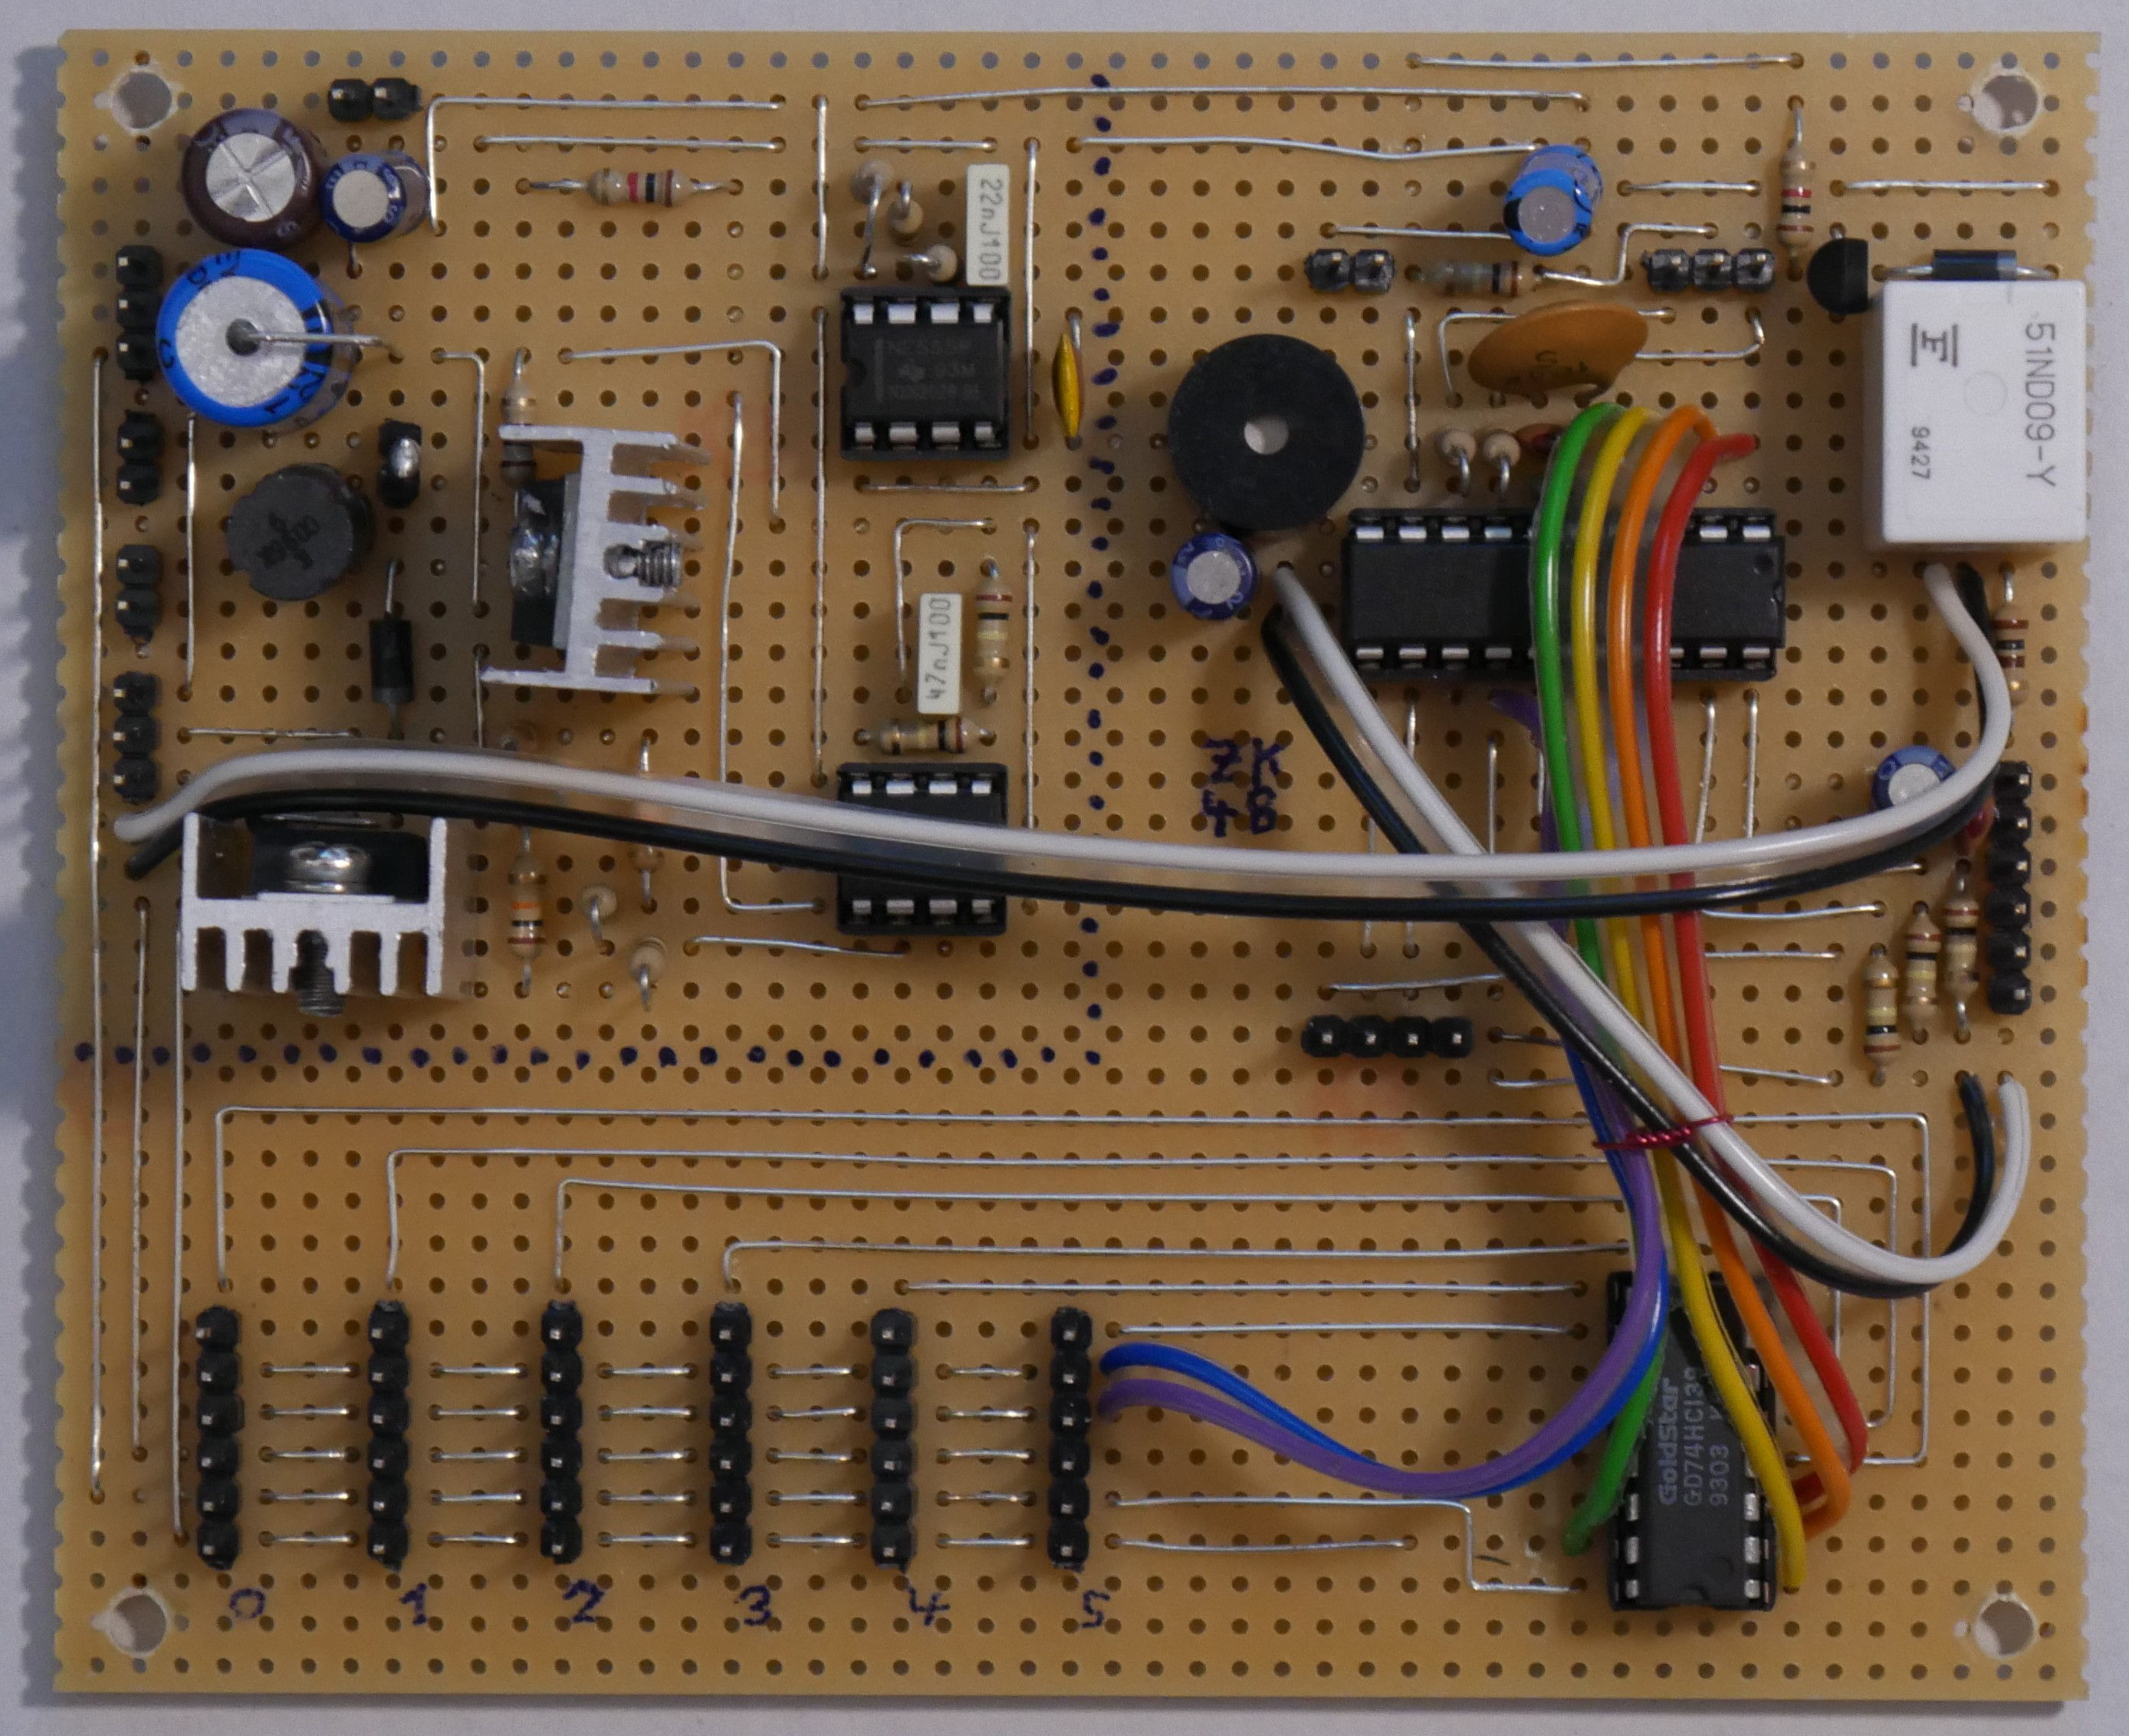
\includegraphics[width=10cm]{./Figures/controller_circuit_soldered.JPG}
    \caption{The controller circuit (See \cref{fig:controller_circuit}) and the ignition voltage generator (See \cref{fig:ivg_circuit}) soldered onto a perfboard.   }
    \label{fig:controller_circuit_soldered}     
\end{figure}

\pagebreak

\subsubsection{Housing of the Controller}
\label{Housing of the Controller}

\noindent The image in \cref{fig:controller_plate_top} shows the controller circuit board with all peripheral items connected. On the top are the two big capacitors that store the ignition and intermediate voltage, secured to the board by a metal band.\\

\begin{figure}[!ht]
    \centering
    \includegraphics[width=10cm]{./Figures/controller_plate_top.JPG}
    \caption{ The circuit board depicted in \cref{fig:controller_circuit_soldered} mounted and wired onto the backside of the devices interface. }
    \label{fig:controller_plate_top}     
\end{figure}

\noindent As the baseplate for the interface, a $2cm$ thick wooden plate was used. Holes were drilled to allow switches, status LED and the sockets to be mounted. Then the plate was spray painted black and everything got screwed on. In \cref{fig:controller_plate_side} the controller circuit board is shown mounted by $1,5cm$ four standoffs. For wiring, ribbon cables were used to connect the switches and other input or output items. The sockets of the trigger and modules were wired to the controller circuit by a 5-line telephone cable\footurl{https://amzn.eu/d/65ZALnq} with shielding. This cable was also the choice for externally connecting the trigger and ignition modules to the controller. 

\begin{figure}[!ht]
    \centering
    \includegraphics[width=10cm]{./Figures/controller_plate_side.JPG}
    \caption{The circuit board depicted in \cref{fig:controller_circuit_soldered} mounted and wired on the backside of the devices interface viewed from the side. }
    \label{fig:controller_plate_side}     
\end{figure}

\pagebreak

\begin{figure}[!ht]
    \centering
    
\includegraphics[width=4cm]{./Figures/gn_case.jpg}
    \caption{ The gun case used for housing the controller. }
    \label{fig:gn_case}     
\end{figure}

\sourceurl{}{fig:gn_case}{https://amzn.eu/d/eWSlyFs}

\noindent A gun case was bought of \textit{Amazon} (See \cref{fig:gn_case}), and the cushioning in the lower part of the case was removed, to make room for the controller. The complete controller/interface was put into a case and screwed in from the sides. \Cref{fig:controller_open} depicts the finished controller powered on. The earlier mentioned lighting(See \cref{Components of the Controller} "Additional circuits") was installed in to top part of the case and the wires were hidden behind the cushioning. In \cref{fig:controller_open} the wires can be seen coming out from the top part of the case and going to the lower part(See \cref{fig:controller_open} right top corner).


\begin{figure}[!ht]
    \centering
    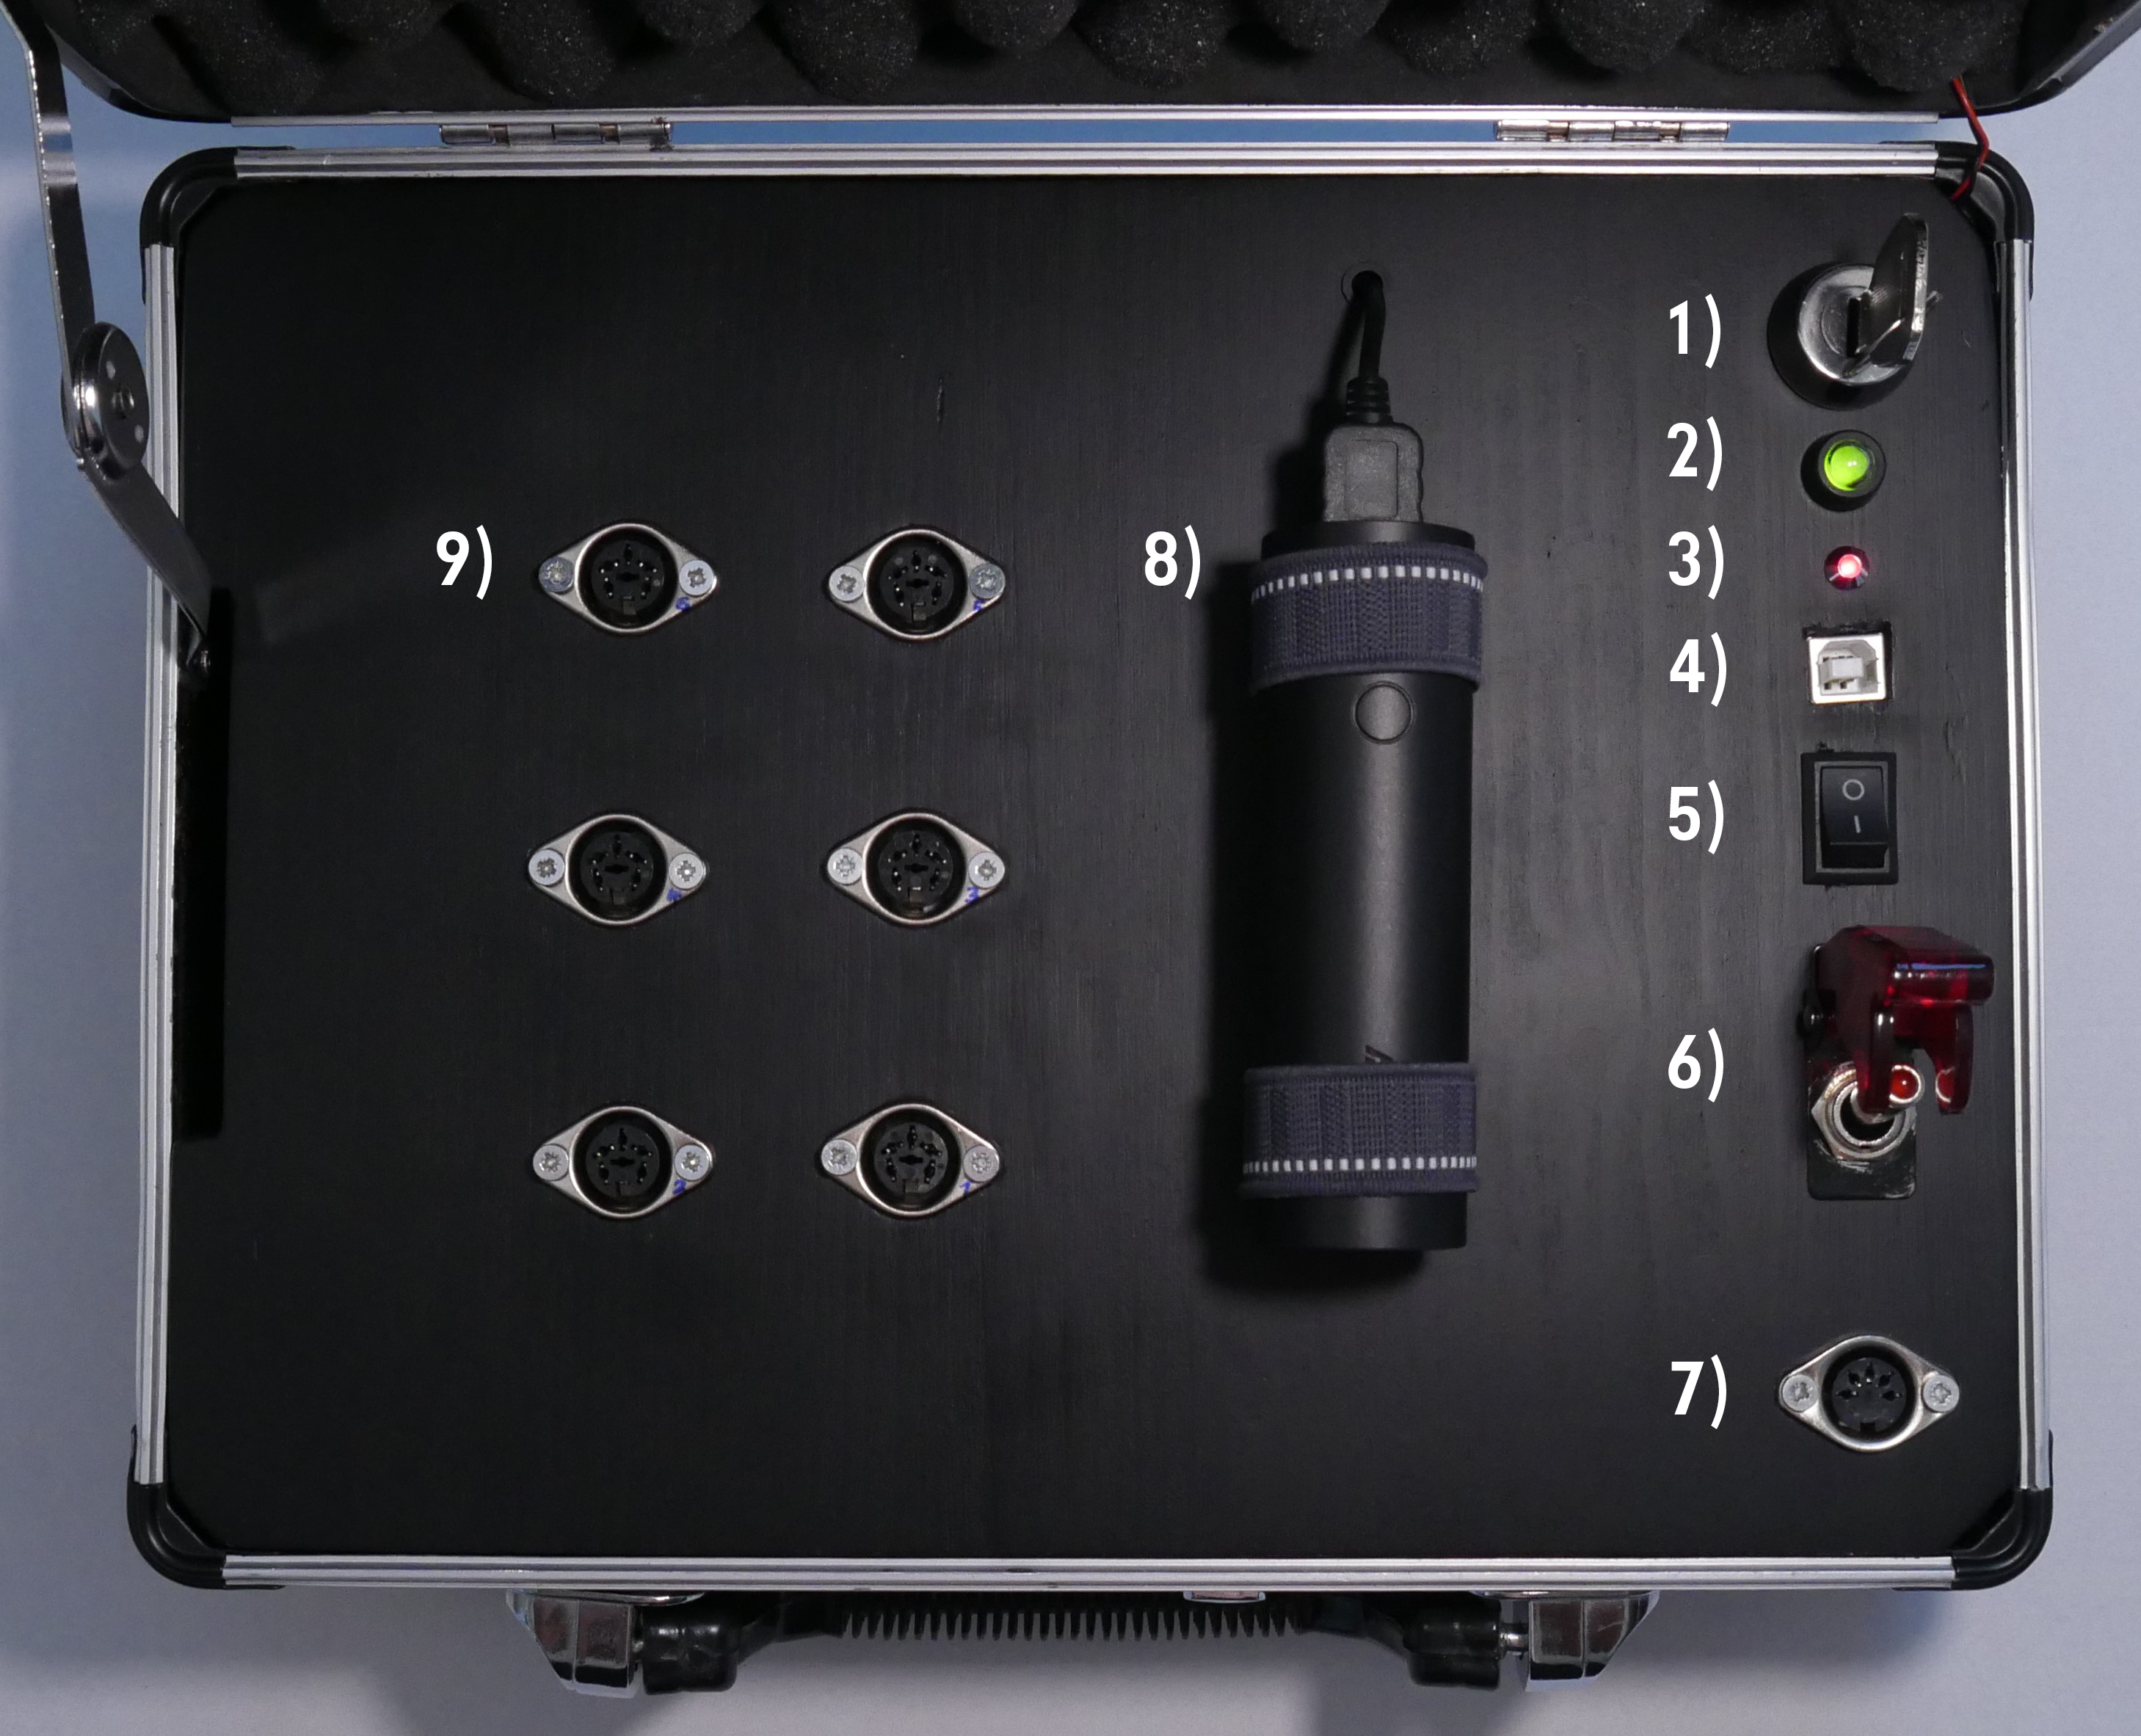
\includegraphics[width=10cm]{./Figures/controller_open_legend.png}
    \caption{ The complete controller and interface inside its case. }
    \label{fig:controller_open}     
\end{figure}

\begin{enumerate}
	\item ON/OFF key-switch
	\item Status LED 
	\item Ignition voltage reached indicator (See \cref{Ignition Voltage Generator})
	\item USB female socket for programming
	\item Light ON/OFF switch
	\item Controller arm switch
	\item Trigger socket
	\item Power bank
	\item Module sockets
\end{enumerate}

\pagebreak

\subsection{Trigger}

\begin{figure}[!ht]
    \centering
    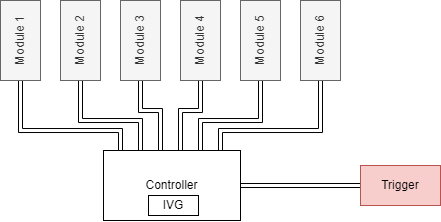
\includegraphics[width=5cm]{./Figures/concept_trigger.png} 
\end{figure}

\noindent The external trigger is responsible for starting the pyrotechnic show. Its purpose is to tell the controller when to start, but also tell the user what the state the controller is currently in. This is very important, because the user must be far away from the controller when the pyrotechnics are ignited, but also needs to be informed if the system is working properly or not.

\subsubsection{Circuit}

\begin{figure}[!ht]
    \centering
    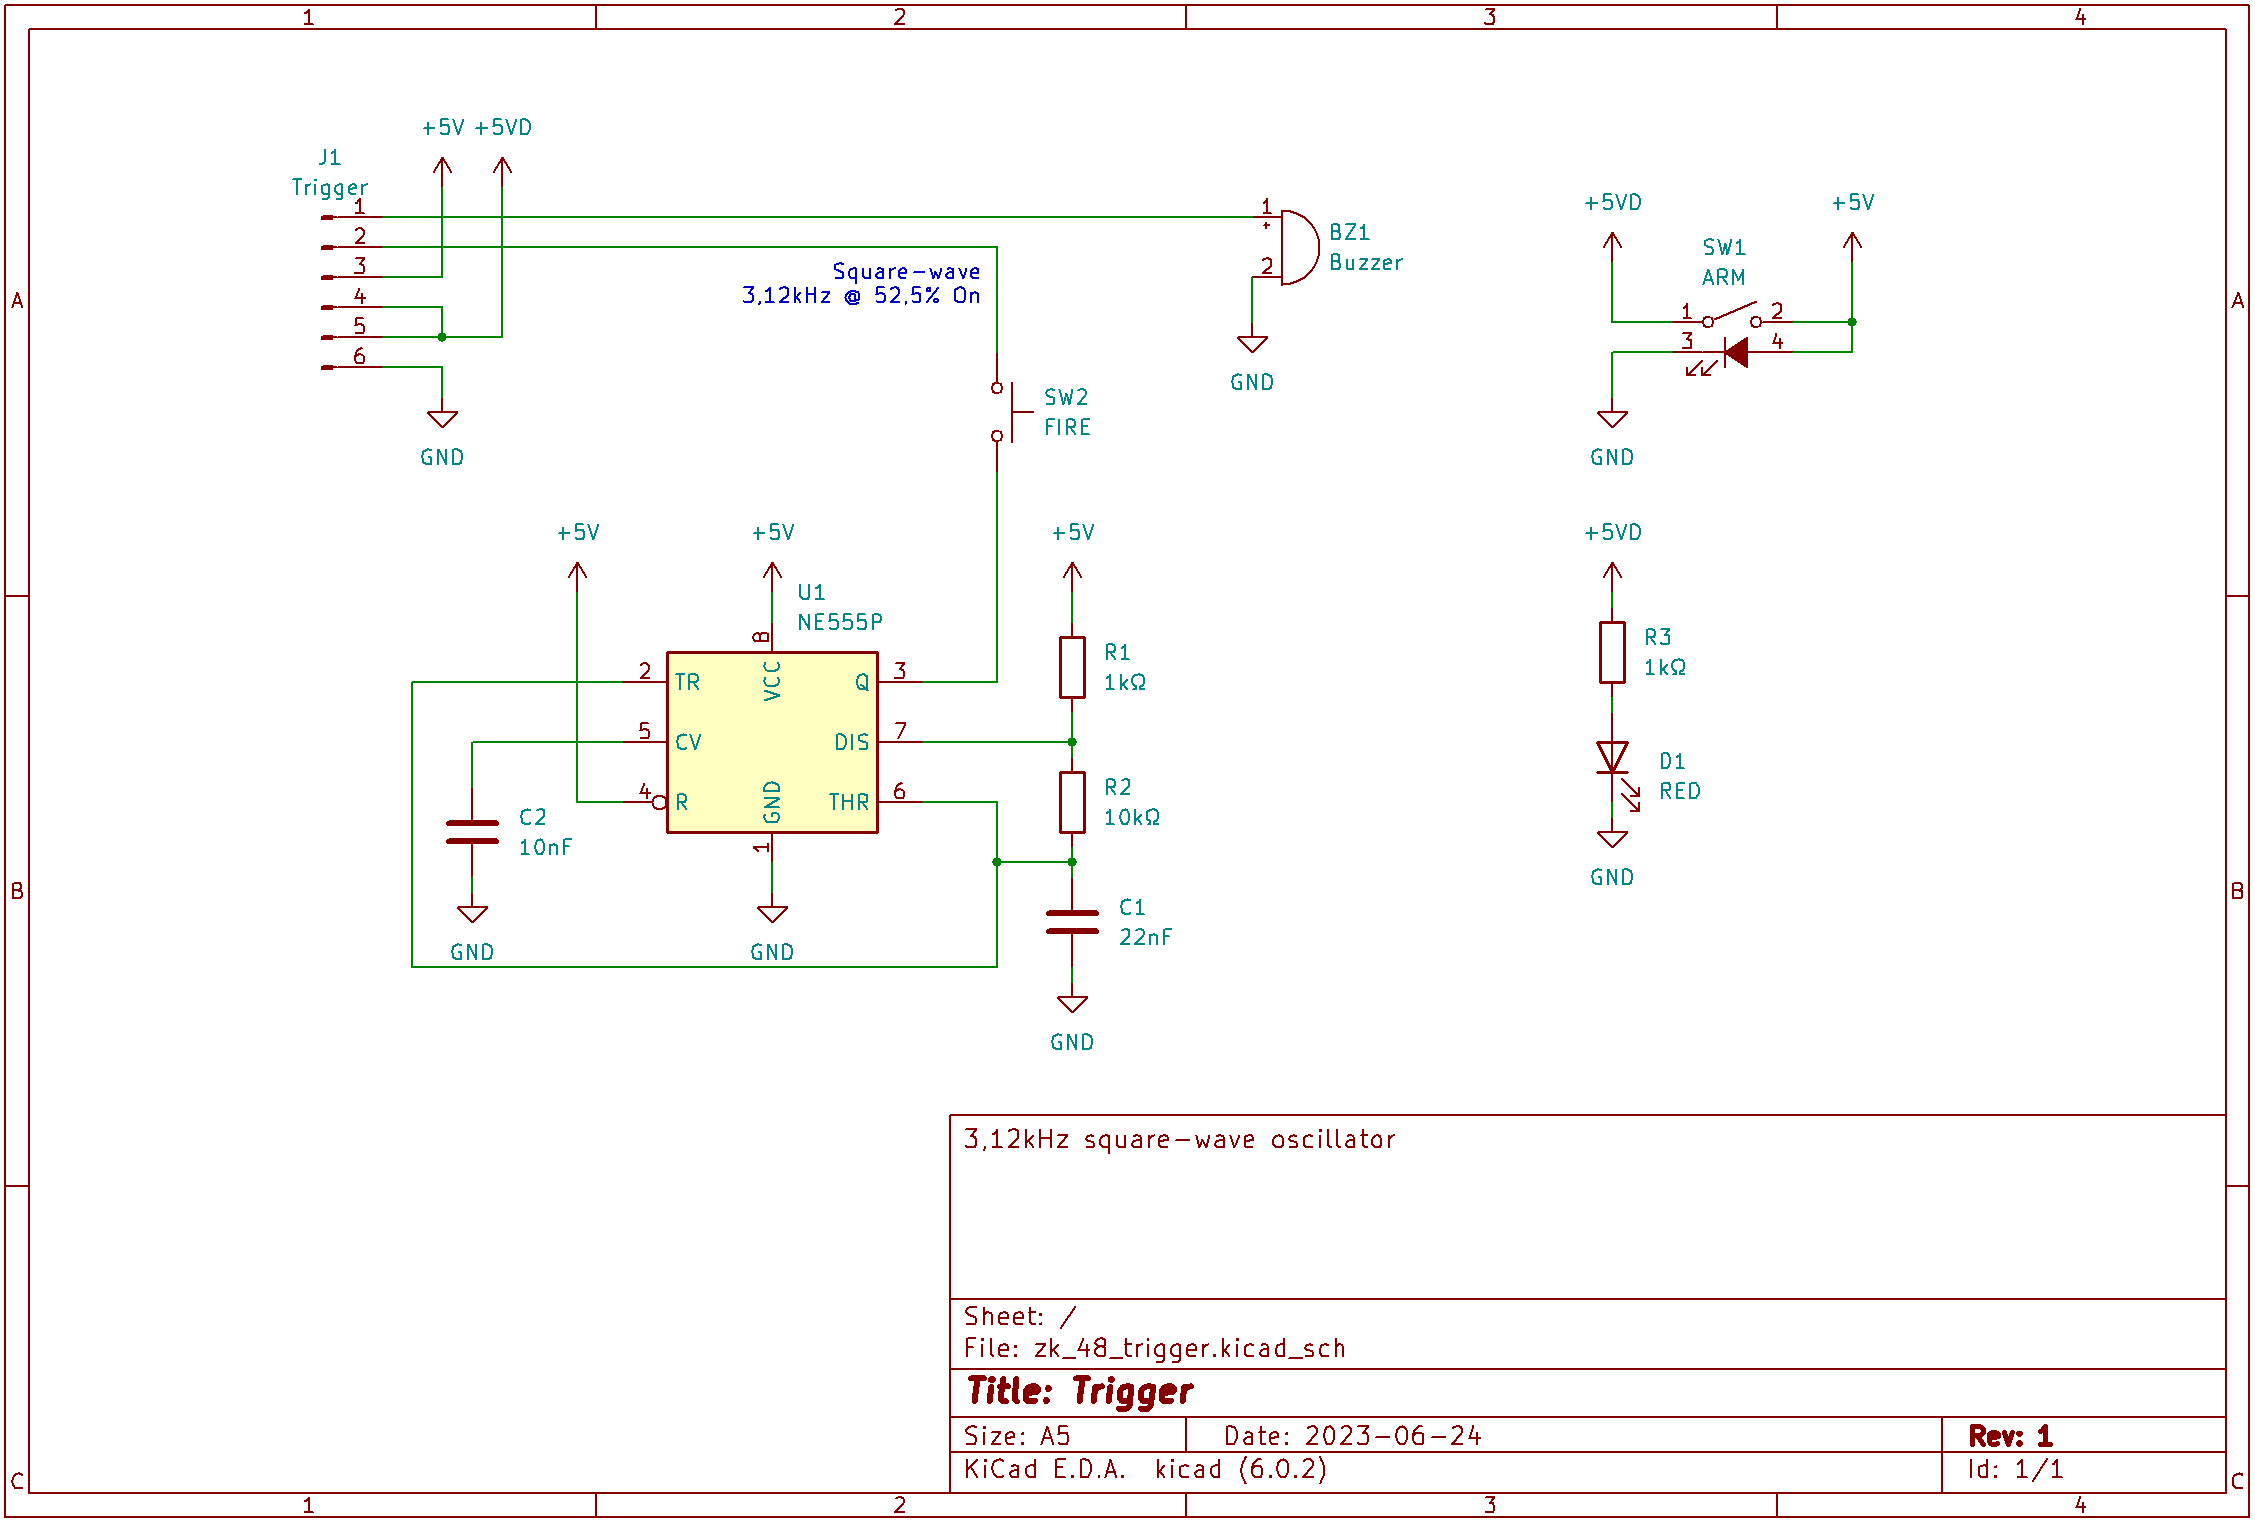
\includegraphics[width=15cm]{./Figures/trigger_circuit.png}
    \caption{The circuit of the external trigger.}
    \label{fig:trigger_circuit}     
\end{figure}

\pagebreak

\subsubsection{How does the trigger work?}
The trigger receives one signal and sends three signals back to the controller. The first input signal is going to buzzer and is also connected to the buzzer on board the controller (See \cref{fig:controller_circuit}). This buzzer gives the user feedback about the systems state, by changing the frequency of the sound produced. But more about the different sound and light outputs in \cref{Firmware}. One of the three outputs is the CONCD signal, which stands for "Connected" and tells the µC if the trigger is plugged in. This output is directly connected to the $+5V$ power line. The second output is the ARMED signal, which indicates to the µC if the trigger is armed. This signal is produced by toggling the arm switch $SW1$ which also turns on the NE555 oscillator. If the trigger is armed, the NE555 will generate a $3,12kHz$ square-wave signal with a $52,2\%$ on-time. This signal is not passed through, until the user holds down the fire $SW2$ button. Then the square-wave signal will be put through on the FIRE line of the trigger, therefore starting the firing sequence. A small LED $D1$ is also present on the trigger to indicate if the trigger has power.


\subsubsection{Housing of the Trigger}

\begin{figure}[!ht]
    \centering
    \includegraphics[width=10cm]{./Figures/trig_open.JPG}
    \caption{The external trigger circuit board mounted inside its case.}
    \label{fig:trig_open}     
\end{figure}

\noindent The circuit diagram of the trigger shown in \cref{fig:controller_circuit}, got soldered onto a small perfboard. Together with the arm switch, power LED and fire button, the circuit was mounted into a ABS housing with the dimensions of $150x45x55mm$ as shown in \cref{fig:trig_open}. The trigger uses a telephone cable, as described in \cref{Housing of the Controller}, with a length of approximately $15m$ to connect to the controller. In \cref{fig:trig_with_cable_legend} the finished controller is visible with the cable and plug.

\begin{figure}[!ht]
    \centering
    \includegraphics[width=10cm]{./Figures/trig_with_cable_legend.png}
    \caption{The external trigger with its cable.}
    \label{fig:trig_with_cable_legend}     
\end{figure}

\begin{enumerate}
	\item Arm switch
	\item Power LED
	\item Fire button
\end{enumerate}

\pagebreak

\subsection{Ignition Modules}
\label{Ignition Modules}

\begin{figure}[!ht]
    \centering
    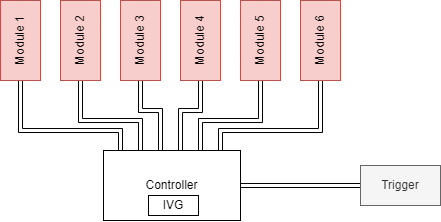
\includegraphics[width=5cm]{./Figures/concept_modules.png} 
\end{figure}

\noindent The ignition modules are responsible for the ignition of the pyrotechnic bridge wire detonators and therefore carry a large responsibility. There is no margin of error, as the whole system depends on the ignition modules proper function. Also the cost of each ignition module must be considered, as six modules need to be build.

\subsubsection{Circuit}

\begin{figure}[!ht]
    \centering
    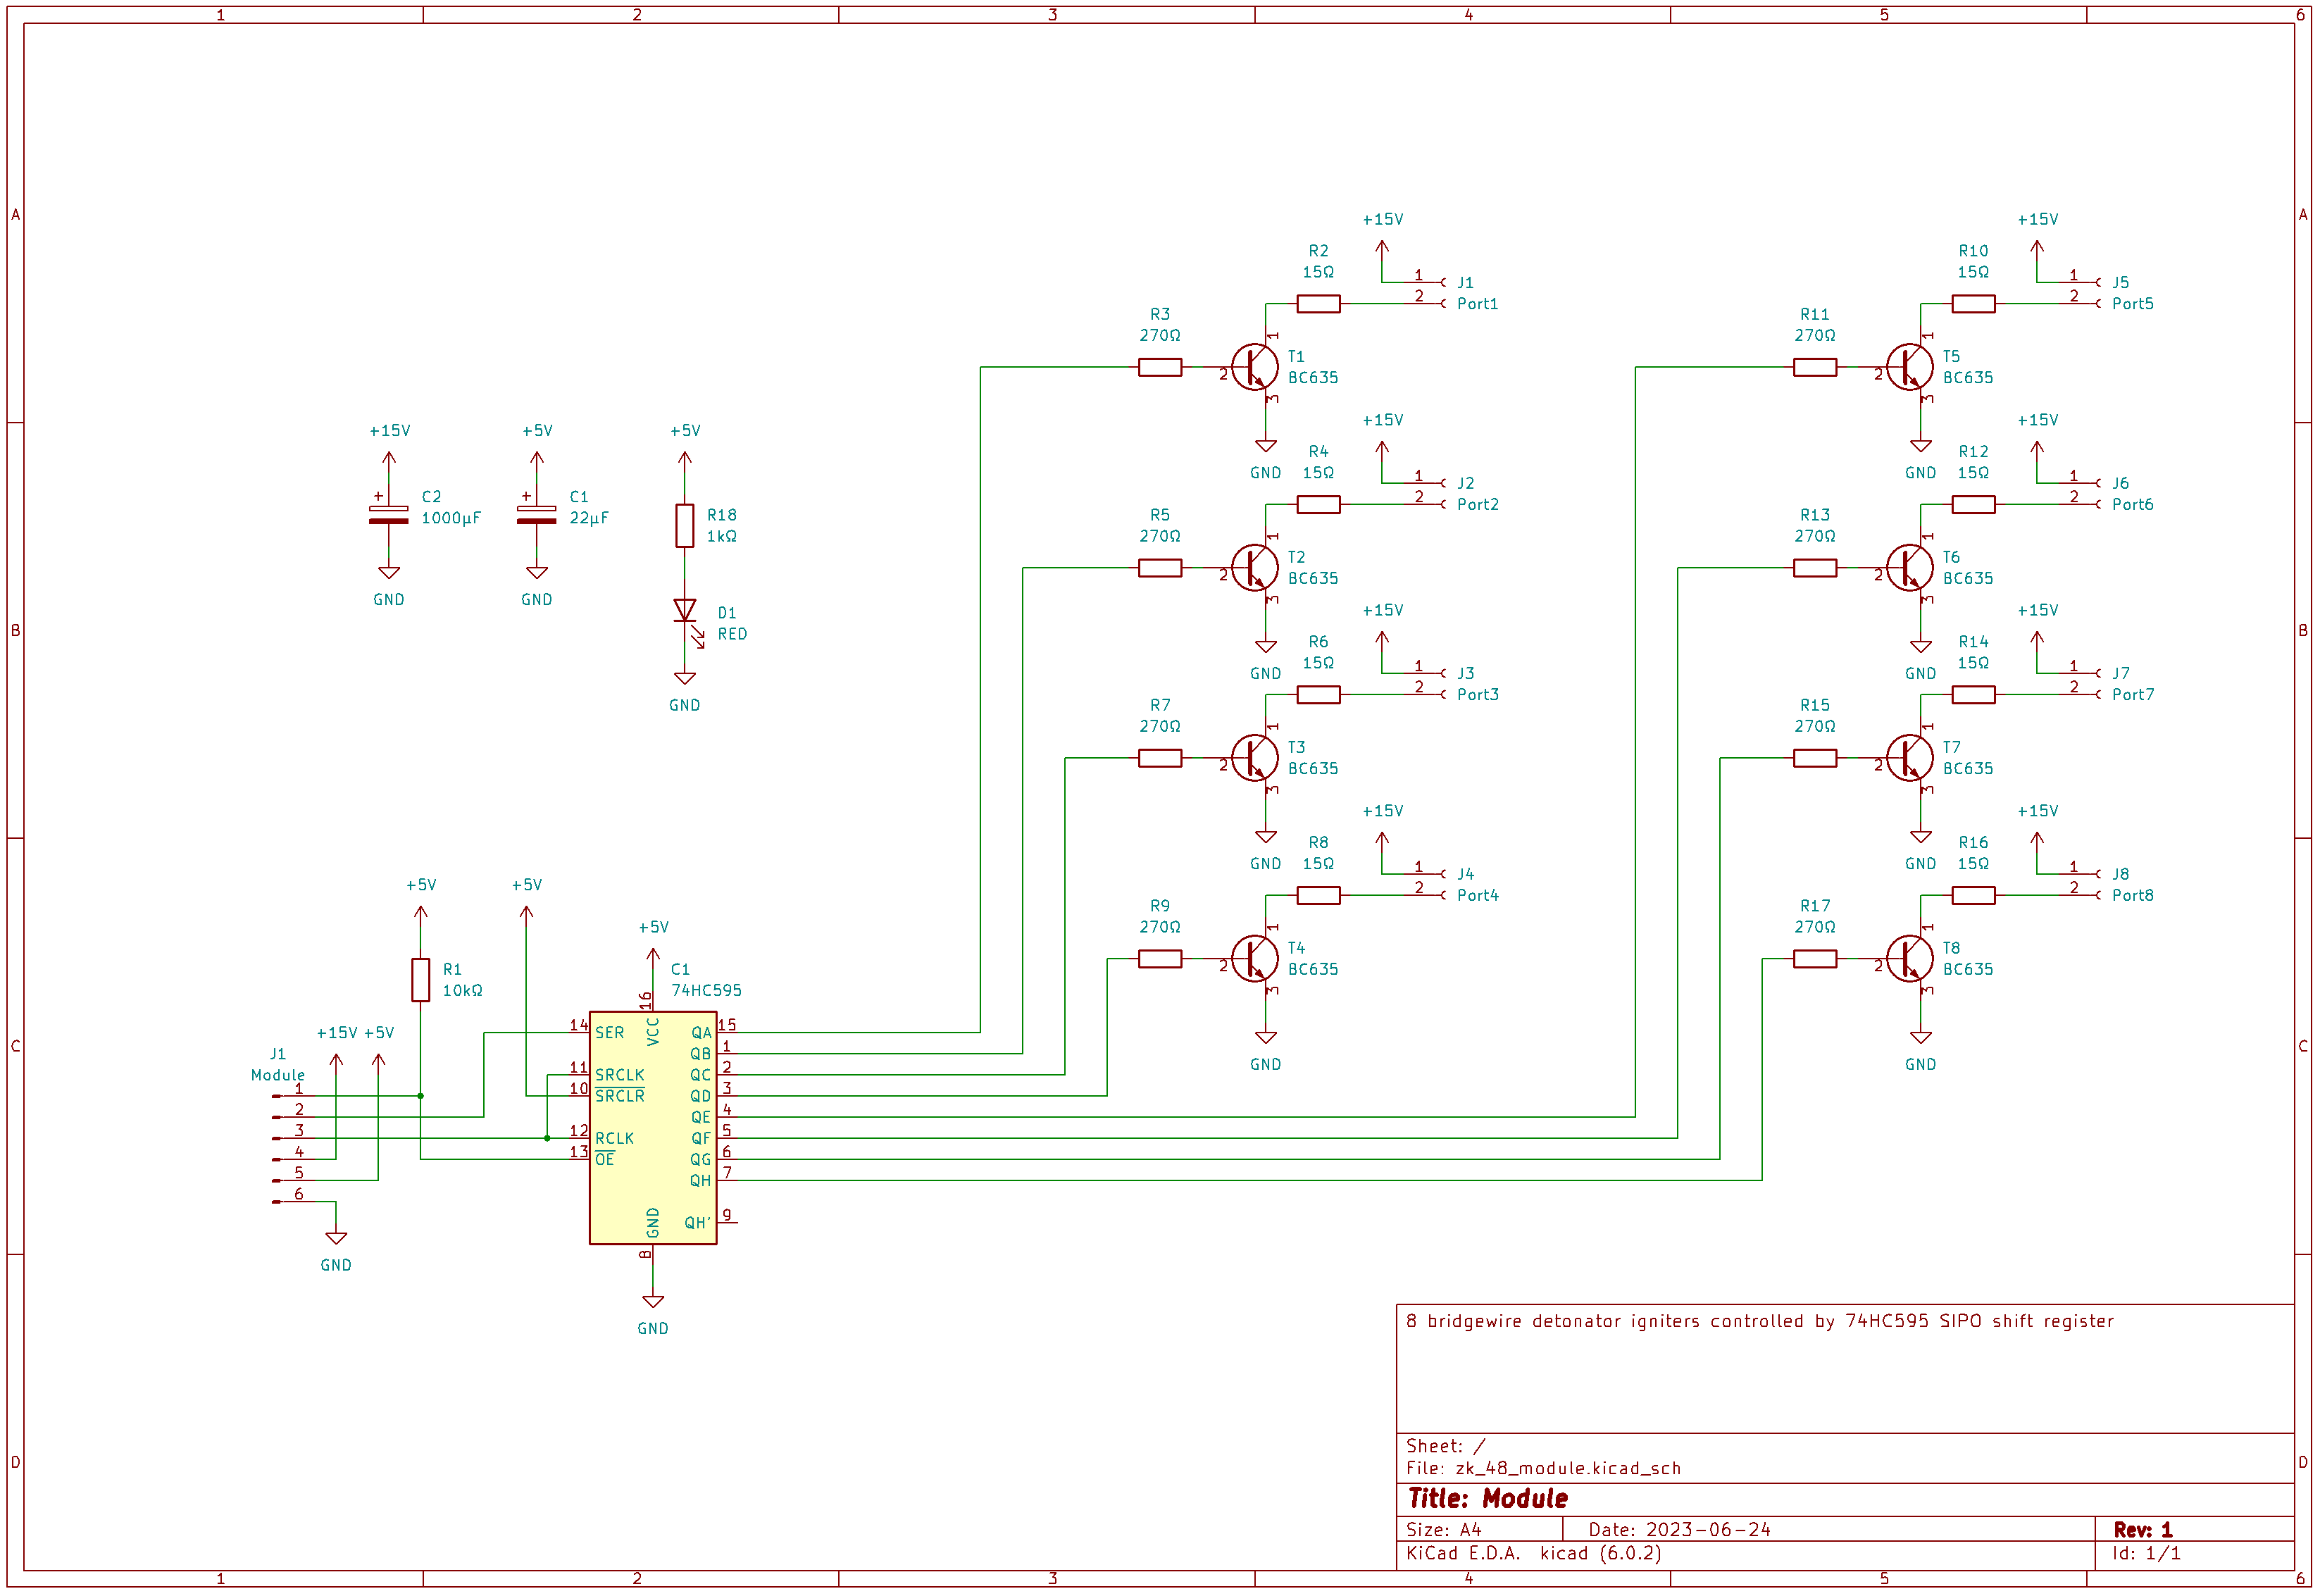
\includegraphics[width=15cm]{./Figures/module_circuit.png}
    \caption{The circuit of the ignition module.}
    \label{fig:module_circuit}     
\end{figure}

\pagebreak

\subsubsection{How does the Ignition Module work?}
\label{Ignition Module work}
\paragraph{Ignition Circuit}

\noindent When setting off a bridge wire detonator, a current larger than $500mA$ must flow, for guaranteed ignition. The switching transistor must therefore be able to handle such currents repeatedly without being damaged. Furthermore, considering that detonators can be faulty, for example have an internal short-circuit, those larger currents should also not destroy the transistor. Additional to the actual electrical requirements, the cost of each module should stay on the lower end, as six modules are going to be build with eight ignition circuits.\\

\begin{figure}[!ht]
    \centering
    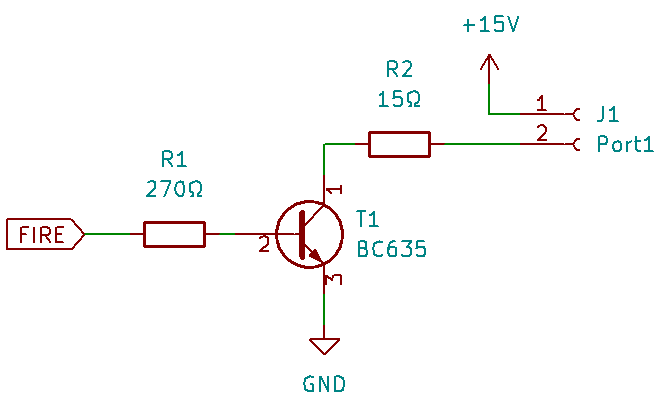
\includegraphics[width=8cm]{./Figures/module_ignitor.png}
    \caption{The circuit designed for setting off one bridge wire detonator inside the ignition module.}
    \label{fig:module_ignitor}     
\end{figure}

\noindent All aforementioned considerations were dealt by limiting the current through the transistor. Limiting the current was accomplished by using a $15\Omega$ resistor after the bridge wire detonator (See \cref{fig:module_ignitor} $R2$) which limits the current, at $15V$ ignition voltage, to maximal $1A$. Knowing the maximal current and considering the other requirements, the NPN transistor BC635\footurl{https://www.tme.eu/Document/aa873a3a455ba8f13e3474bd76bcc1d9/BC635_40.pdf} in a TO-92 package, was chosen as the switching transistor. Its continuous collector current is equal to $1A$ and a costs 0,09€ per piece. To drive the BC635 a $270\Omega$ resistor was used to limit the base current to circa $16mA$ (See \cref{eq:base_current}), which results in the saturation of the transistor. \Cref{fig:module_ignitor} displays the complete ignition circuit.

\begin{equation}
I_B=\frac{U_{IC,OUT}-U_{BE}}{R}=\frac{5V-0,7V}{270\Omega}=15,93mA
\label{eq:base_current}
\end{equation}\\

\noindent Designing this circuit also required selecting the proper ignition voltage level. The reason why the ignition voltage is $15V$ and not $5V$, which would make things much simpler, can be explained by Ohm's law: If the ignition voltage is $5V$ instead of $15V$ and the current is still gets limited to $1A$ by a $5\Omega$ resistor, a reduction of the current through the detonator will occur. The calculations below (\Cref{eq:current_15v} and \cref{eq:current_5v}) calculate the current for both cases, by simulating a bridge wire detonator with the same resistor value of $4,7\Omega$ as used in \cref{Testing}.

\begin{equation}
I=\frac{U_{IG}}{R_2+R_{BWD}}=\frac{15V}{15\Omega+4,7\Omega}= 761,14mA
\label{eq:current_15v}
\end{equation}\\
\begin{equation}
I=\frac{U_{IG}}{R_2+R_{BWD}}=\frac{5V}{5\Omega+4,7\Omega}= 515,54mA
\label{eq:current_5v}
\end{equation}\\

\noindent Comparing result of \cref{eq:current_15v} to result of \cref{eq:current_5v}, a strong drop in current is noticeable. This is a problem that worsens with additional detonators connected. In a typical pyrotechnic show it is not unlikely for three or more detonators to be connected in series(Parallel wiring is not recommend in general). A stronger transistor could be used, but this would raise cost, which is unwanted as 48 transistors are required.\\

\pagebreak

\paragraph{Controlling the Ignition Circuits}
As mentioned in previous sections, the modules are based on a 8-Bit SIPO (Serial-in Parallel-out) shift register 74HC595\footurl{https://www.ti.com/lit/ds/symlink/sn74hc595.pdf}. 

\begin{figure}[!ht]
    \centering
    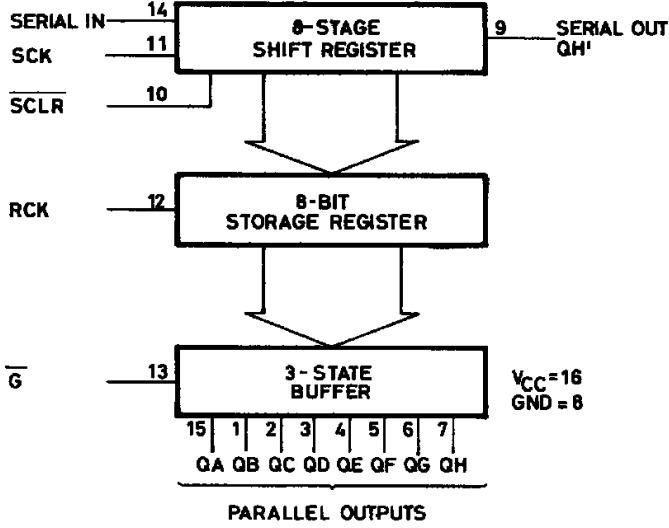
\includegraphics[width=8cm]{./Figures/75hc595_functional.png}
    \caption{Functional diagram of the 74HC595}
    \label{fig:75hc595}     
\end{figure}

\sourceurl{}{fig:75hc595}{https://cdn-reichelt.de/documents/datenblatt/A240/74HC595\%23STM.pdf}

\noindent The 74HC595 is made up of three subcomponents: the shift register, a register and a tri-state buffer(See \cref{fig:75hc595}). To fire a port, the µC sends a byte mask serially to the shift-register (In \cref{fig:75hc595} see pin 14 SERIALIN and 11 SCK) where only one bit is set, indicating which port is being fired. Because the register clock RCK and shift register clock SCK are wired together (See \cref{fig:module_circuit}) the register will take on the values from the shift register. As also mentioned in \cref{Components of the Controller} "Peripheral Managing and Controlling Logic" the µC afterwards selects the correct module being fired by pulling low of the enable pin on the tri-state buffer (pin 13 in \cref{fig:75hc595}), thus outputting the stored bit mask of the register onto the parallel outputs. \Cref{fig:module_circuit} shows that each output is directly connected to one ignition circuit, whereby the setting of an output to logic high fires a detonator.\\

\paragraph{Additional circuits}
To reduce the large ignition currents through the cable which could cause interference in the signal lines, a large $1000 \mu F$ capacitor $C_2$ was added to the $15V$ ignition voltage line inside the ignition module (See \cref{fig:module_circuit}). As charge would be stored closer to detonator theoretically this should in theory reduce peak currents, however this is speculative and the capacitor might not be needed at all.\\

\pagebreak

\subsubsection{Housing of the Ignition Modules}

\noindent The circuit got soldered onto a perfboard and for the housing a common electrical junction box, from the hardware store, was used as it is cheap, light weight, easy to cut and can be screwed against something. For connecting to the controller, four pieces of $4m$ and four pieces of $8m$ telephone cables were cut to size and soldered to the each of the eight modules circuit boards as seen in \cref{fig:mod_open}. Also visible in \cref{fig:mod_open} is the orange stabilizing $1000 \mu F$ capacitor $C2$ seen in \cref{fig:module_circuit}.

\begin{figure}[!ht]
    \centering
    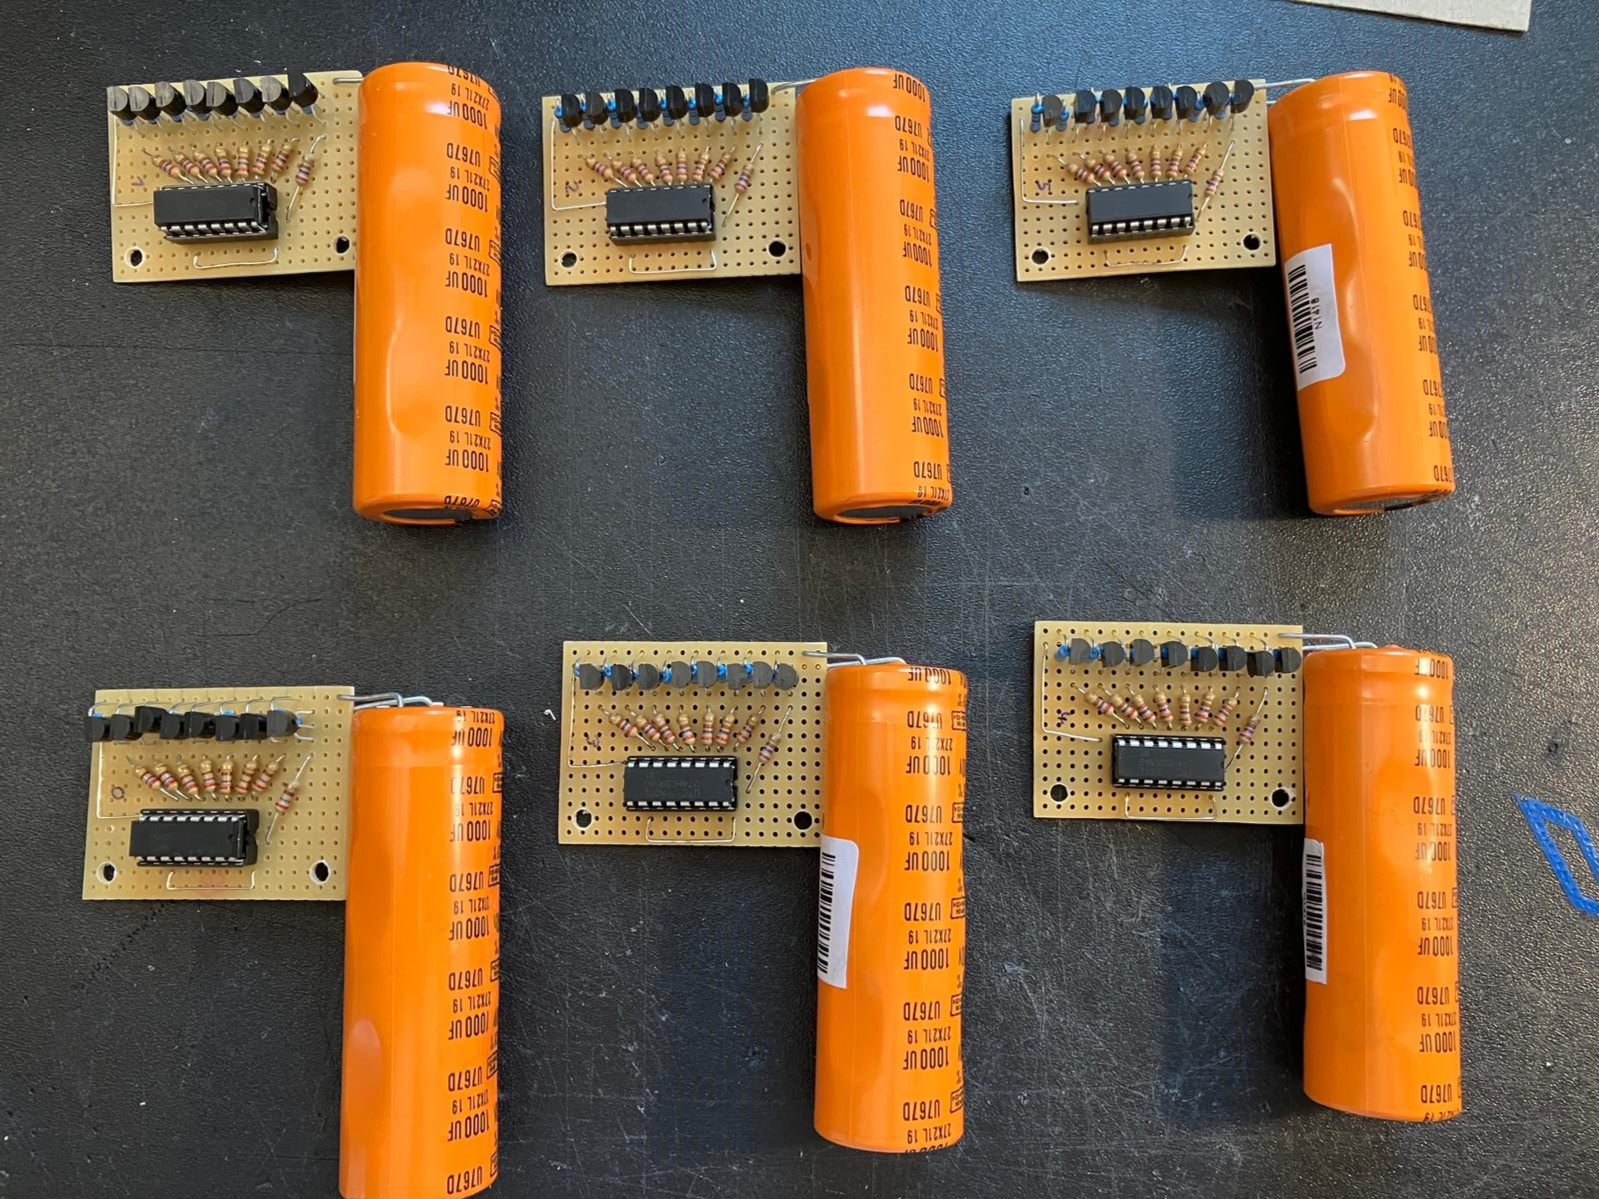
\includegraphics[width=7cm]{./Figures/raw_modules.jpeg}
    \caption{All six ignition modules soldered onto perfboards.}
    \label{fig:raw_modules}     
\end{figure}

\noindent To connect the bridge wire detonators to the circuit, speaker terminals were used.  In \cref{fig:mod_closed} the bottom two terminal rows represent the eight ports and the top row are all $15V$. This design is less ideal, because for two ports there is only one $15V$ terminal hole, but due limited space on top the housing this was a necessary compromise.  \\

\begin{figure}[!ht]
    \centering
    \includegraphics[width=7cm]{./Figures/mod_closed.JPG}
    \includegraphics[width=7cm]{./Figures/mod_open.JPG}
    \caption{The ignition module from the inside (right) and the complete moudle with eight ports on the bottom and one power rail on the top (left).}
    \label{fig:mod_open}     
\end{figure}

\pagebreak
